\documentclass[a4paper,12pt,oneside]{article}


\usepackage{color}
\usepackage[margin=1in]{geometry}
\usepackage{float}
\usepackage{sectsty}
\usepackage{graphicx}
\usepackage{enumitem}

\usepackage{tikz}



\title{Algérienne Démocratique et Populaire\\
Ministère de l’Enseignement Supérieur et de la Recherche
Scientifique}



\begin{document}

\begin{titlepage}

    \centering
    \vfill
{\bfseries\Large
        République Algérienne Démocratique et Populaire 
		Ministère de l’Enseignement Supérieur et de la Recherche
		Scientifique\\
		\vskip1cm
		\hrule


		\begin{center}
		
		
\includegraphics[width=0.5\textwidth]{ESTIN-LOGO}
		
		\end{center}
		
		
  		

		
        École supérieure en Sciences et Technologies\\
        de l'Informatique et du Numérique\\
        
        \vskip1cm
        {\Huge RAPPORT DE PROJET :}\\
        \vskip1cm
        Thème :\\ Plateforme de gestion d'un magasin de plantes\\
        \vskip1cm
        Ce projet est réalisé par : \\
        
  		
  		\begin{itemize}
    		\item[]
    		\begin{minipage}[t]{0.05\linewidth}
        $\bullet$
    		\end{minipage}
    		\begin{minipage}[t]{0.45\linewidth}
        CHAREF Amir
    		\end{minipage}
    		\begin{minipage}[t]{0.05\linewidth}
        $\bullet$
    		\end{minipage}
    		\begin{minipage}[t]{0.45\linewidth}
        BAHLOUL Rami 
    		\end{minipage}
    		\begin{minipage}[t]{0.05\linewidth}
        $\bullet$
    		\end{minipage}
    		\begin{minipage}[t]{0.45\linewidth}
        BOUHAFS Imane
    		\end{minipage}
    		\begin{minipage}[t]{0.05\linewidth}
        $\bullet$
    		\end{minipage}
    		\begin{minipage}[t]{0.45\linewidth}
        MAKHLOUF Sanad
    		\end{minipage}
    		\item[]
    		\begin{center}
         $\bullet$  DJENNANE Khadidja
    		\end{center}
    		
		\end{itemize}
		
		\vskip1cm
	
        Encadré par : \\
        \begin{itemize}
        \item[]
    		\begin{center}
         $\bullet$  Mlle AGGAOUA MERIEM
    		\end{center}
    		\item[]
    		\begin{center}
         $\bullet$  Mlle Nawel ARAB
    		\end{center}
    		\end{itemize}
        \vspace*{\fill} 
        \vfill
        Année universitaire : 2022-2023\\   
}
\end{titlepage}


\newpage
\begin{center}
{\bfseries\Large
{\Huge REMERCIEMENTS :}\\
}
\end{center}
\vskip1cm

{\fontsize{16}{20}\selectfont
En tout premier lieu, nous remercions le bon Dieu, tout puissant,
de nous avoir donné la force pour survivre, ainsi que l’audace
pour dépasser toutes les difficultés. Permis de mener `a bien ce
projet. Louange à ALLAH le tout puissant.
\vskip2mm
Nous tenons à remercier chaleureusement toutes les personnes qui ont contribué à la réalisation de ce projet de gestion d'un jardin de plantes.
\vskip2mm
Nous adressons nos plus sincères remerciements à nos chères
encadreuses Mlle Nawel ARAB et Mlle Aggaoua MERIEM pour la richesse et la qualité de leur encadrement , pour tous leurs précieux conseils,pour leurs écoutes actives et leurs disponibilités tout au long de la réalisation de ce projet.
\vskip2mm
Nous souhaitons également adresser nos remerciements aux membres de l'équipe de ce projet, pour leur disponibilité et leur collaboration tout au long de la réalisation de ce projet. Leur expertise nous a été précieuse et a grandement contribué à la qualité de notre travail.
\vskip2mm
Enfin, nous tenons à remercier nos familles et nos amis pour leur soutien inconditionnel, leur patience et leur compréhension durant cette période intense de travail.
\vskip2mm
Nous sommes conscients que ce projet n'aurait pas été possible sans l'implication de chacun de ces acteurs et nous leur exprimons notre sincère gratitude.
}

\newpage
\tableofcontents
\newpage
\listoffigures
\newpage
\listoftables

\newpage




\section{Introduction générale :}

{\fontsize{15}{20}\selectfont 

\hspace{1cm}La gestion d'un jardin de plantes est une tâche complexe qui nécessite une planification minutieuse, une connaissance approfondie des plantes et de leur environnement, ainsi qu'une gestion efficace des ressources disponibles. Dans un contexte où la protection de l'environnement et le développement durable sont devenus des enjeux majeurs, la gestion d'un jardin de plantes doit également intégrer ces préoccupations pour garantir un avenir viable et respectueux de la nature.
\vskip1mm

Dans ce rapport, nous présentons notre travail sur la conception et la réalisation d'une plateforme de gestion d'un jardin de plantes pour le jardin de \textbf{OUCHEN AHCENE}. Notre plateforme a été conçue pour répondre aux défis rencontrés par les gestionnaires de ce jardin, qui doivent aujourd'hui faire face à des enjeux complexes et diversifiés. Elle propose des solutions innovantes pour optimiser la gestion du jardin, tout en prenant en compte les critères de durabilité et de respect de l'environnement propres à ce jardin.

La réalisation de cette plateforme soulève plusieurs questions auxquelles nous tenterons de répondre tout au long de ce rapport. Quelles sont les fonctionnalités indispensables à inclure dans une plateforme de gestion d'un jardin de plantes ? Comment garantir la sécurité des données des utilisateurs de la plateforme ? Comment assurer une utilisation intuitive et conviviale de l'interface ? Quels sont les enjeux environnementaux liés à la gestion d'un jardin de plantes et comment peuvent-ils être pris en compte dans la plateforme ?
\vskip1mm

Dans une première partie, nous présentons les objectifs et les enjeux de notre projet pour le jardin , ainsi que les méthodes et les outils que nous avons utilisés pour le réaliser. Nous détaillons ensuite les différentes fonctionnalités de la plateforme, en mettant en avant les avantages qu'elles apportent aux gestionnaires du jardin. Enfin, nous concluons en présentant les perspectives d'avenir de notre plateforme pour ce jardin, ainsi que les limites et les axes d'amélioration possibles.
\vskip1mm

Notre travail de conception et de réalisation de cette plateforme  s'inscrit dans une démarche d'innovation et de développement durable, qui vise à répondre aux enjeux spécifiques de ce jardin. Nous espérons que ce rapport contribuera à la diffusion de ces innovations et à la promotion d'une gestion responsable et durable de l'environnement végétal du jardin .
\vskip1mm

Ce rapport est structuré en trois chapitres distincts qui abordent les différentes étapes de la réalisation de notre plateforme de gestion de jardin de plantes.
\vskip1mm

Le premier chapitre, intitulé "Spécification des besoins", se focalise sur la compréhension des attentes de notre client ainsi que sur l'analyse des besoins fonctionnels et non fonctionnels de la plateforme. Nous y présenterons également une étude de l'existence ainsi que des critiques afin de mieux appréhender les enjeux et les opportunités liées à notre projet.
\vskip1mm

Le deuxième chapitre, intitulé "Conception", se concentre sur la modélisation de la plateforme. Nous y décrirons les différents diagrammes de séquence et de classe ainsi que le modèle relationnel. Cette étape est cruciale pour assurer une implémentation efficace de la plateforme.
\vskip1mm

Le troisième chapitre, intitulé "Réalisation", met en évidence les outils de développement utilisés et décrit en détail les fonctionnalités de la plateforme. Nous y présenterons des captures d'écran pour illustrer les différents aspects de notre solution.
\vskip1mm

Enfin, le rapport sera clôturé par une conclusion générale qui synthétisera les différents apports de notre plateforme de gestion de jardin de plantes. Nous y présenterons également une bibliographie/webographie ainsi qu'un résumé/traduction pour faciliter la compréhension de notre travail.
\vskip2mm

Nous avons vu l’introduction générale et nous avons présenté
la problématique et les solutions proposées, alors passons au contenus des chapitres ...

}

\newpage

\section{CHAPITRE 01 : Spécification des besoins}
{\fontsize{15}{20}\selectfont 
\subsection{Introduction}

\hspace{1cm}Notre projet nécessite une phase d’analyse et
de conception, dans lesquelles nous allons
décrire de façon précise les besoins des
utilisateurs et des clients.
A ce stade du projet on se pose des questions :
Qui est notre client ? Quelles sont les
problématiques et leurs solutions ? Quelles sont
les besoins du client et nos propositions ? et quel
est notre objectif dans cette plateforme ?
Dans ce chapitre, on s’intéresse à apporter des
réponses précises avec des détails aux
questions déjà posées en clarifiant leurs aspects
techniques.
\textbf{PLANTEX} est une plate-forme qui représente un
grand jardin qui fournit des informations sur les
services de jardinage, des conseils de jardinage,
des idées d'aménagement paysager et des
produits de jardinage disponibles à l'achat.

\subsection{Présentation du client}

\hspace{1cm}Notre client c'est le responsable de cette jardin.
Monsieur OUCHEN AHCENE est une personne qui
travaille dans une pépinière, un magasin de
jardinage ou une jardinerie et qui est chargée de
vendre des plantes, des arbres, des arbustes et
des accessoires de jardinage aux clients, situé à "
Route Village Agricole, Souk El Ténine,Béjaia ".\\
\textbf{Ses responsabilités en générale sont :}

\begin{enumerate}
\item Accueil et conseil des clients : Mr OUCHEN
accueille les clients, répond à leurs questions
et les conseille sur les différentes variétés de
plantes et d'arbres disponibles, en fonction
de leurs besoins et de leurs préférences.
\item Entretien des plantes : Le vendeur de plantes
veille à ce que toutes les plantes et les arbres
du magasin soient bien entretenus et en
bonne santé, afin d'attirer les clients et de
leur donner confiance dans la qualité des
produits proposés
\item Gestion des stocks : Le vendeur de plantes est
responsable de la gestion des stocks,en veillant à ce que le magasin dispose toujours
des plantes et des arbres les plus populaires et
en commandant de nouveaux stocks lorsque cela
est nécessaire
\item Vente et encaissement : il est chargé de la
vente et de l'encaissement des produits vendus
aux clients, en utilisant un système de caisse
électronique ou manuel.
\item  Promotion des ventes : il peut également
être chargé de promouvoir les ventes en
organisant des événements spéciaux, des
démonstrations et des offres promotionnelles
pour attirer les clients.\\
        \vskip2mm

\textbf{OUCHEN AHCENE} a pour expérience de 10 ans
dans ce domaine des plantes , il sait bien les
conditions nécessaires de chaque arbre, chaque
plantes et chaque article existe dans son
magasin ( outils , engrais ... ) .

\end{enumerate}

\subsection{Pourquoi nous a-t-il choisis ?}
\hspace{1cm}Car tout simplement , on a lui proposer des
fonctionnalités qui en font le meilleur dans le
marché : un Nom commerciale \textbf{PLANTEZ} , un logo
de travail.\\
De plus on a lui proposer un simple UI/UX simple, facile à
utiliser par tout le monde .
}

\subsection{Problématiques/solutions}
\subsubsection{Problématiques}
\begin{itemize}
\item[]
       	 $\bullet$ Saisonnalité : La vente de plantes est souvent
saisonnière, ce qui signifie que les périodes de
forte demande peuvent être limitées à
certaines saisons de l'année, comme le
printemps et l'été. Cela peut poser des
problèmes de gestion des stocks et de
planification des ventes.
\vskip1mm
       	 $\bullet$ Gestion des stocks : Les plantes ont une durée
de vie limitée et nécessitent des soins
spécifiques pour maintenir leur qualité. La
gestion des stocks peut donc être un défi, en
particulier si les plantes ne se vendent pas
rapidement ou si elles sont endommagées
pendant le transport ou le stockage.\\
\vskip1mm
       	 $\bullet$ La majorité des personnes n'arrivent pas à
distinguer entre les différentes types des
plantes et l'environnement qui le faut pour
leurs réussite ( l'eau, la chaleur et la terre ... )\\
Par exemple : si une plante a l'habitude de n'a pas
s'exposer directement à la lumière naturelle , si on
la fait sortir elle ne va pas s'adapter avec ce
changement.\\
\vskip1mm
    		$\bullet$ Concurrence : Les magasins de plantes peuvent
être confrontés à une forte concurrence locale,
en particulier dans les zones urbaines où il y a
de nombreux magasins de jardinage. La
concurrence peut également provenir de la
vente en ligne de plantes, qui peuvent être
moins chères et plus pratiques pour certains
clients. \\
\vskip1mm
    		$\bullet$ Marketing et publicité : Les magasins de
plantes doivent investir dans le marketing et la
publicité pour se démarquer de la concurrence
et attirer les clients. Cela peut inclure la
publicité en ligne, les promotions spéciales, les
événements en magasin, la création d'une
marque forte et la mise en place d'un
programme de fidélité pour les clients
réguliers.\\
\vskip1mm
    		$\bullet$ Gestion des coûts : Les coûts associés à la
gestion d'un magasin de plantes peuvent être
élevés, notamment en ce qui concerne le
transport, le stockage, l'achat de plantes et la
rémunération du personnel.\\
\vskip1mm
    		$\bullet$ Due au occupations de la majorité des
personnes dans leurs vies quotidiennes (
Etudiants , Travailleurs ..) , ils n'ont pas la
capacité ni pour visualiser le produit ni pour
l'acheter .
    		
\end{itemize}


\subsubsection{Solutions}
		\begin{itemize}
        \item[]
       	 $\bullet$ Diversification des produits : Le magasin peut
proposer une large gamme de produits, y
compris des plantes d'intérieur et d'extérieur,
des plantes d'hiver, des outils de jardinage, des
engrais, des pots et des accessoires. Cela
permettra de répondre aux différents besoins
et préférences des clients, tout en attirant une
clientèle plus diversifiée.
\vskip1mm
       	 $\bullet$ Mise en place d'un programme de fidélité : Le
magasin peut proposer un programme de
fidélité pour récompenser les clients réguliers
et encourager la fidélité à long terme. Des
offres spéciales, des remises et des avantages
exclusifs peuvent être proposés aux clients
fidèles pour les inciter à revenir.\\
\vskip1mm
       	 $\bullet$ Marketing et publicité efficaces : Le magasin
peut développer une stratégie de marketing et
de publicité efficace, en utilisant des médias
sociaux, des publicités en ligne, des
événements en magasin, des newsletters, des
brochures et des affiches.Le but est d'attirer une clientèle plus large et de renforcer la notoriété du magasin.\\
\vskip1mm
    		$\bullet$ Amélioration de l'expérience client : Le magasin
peut améliorer l'expérience client en créant un
environnement accueillant et agréable, en
proposant des conseils personnalisés et en
offrant un service client exceptionnel. Des
initiatives telles que des journées portes
ouvertes, des ateliers de jardinage et des
événements communautaires peuvent
également contribuer à renforcer les liens avec
les clients. \\
\vskip1mm
    		$\bullet$ Amélioration de la gestion des stocks : Le
magasin peut améliorer la gestion des stocks
en utilisant des logiciels de gestion des stocks,
en établissant des relations solides avec les
fournisseurs pour s'assurer d'un
approvisionnement régulier en plantes de
qualité et en rationalisant les processus de
stockage et d'achat. Cela permettra de
minimiser les pertes et d'optimiser les profits.\\
\vskip1mm
    		$\bullet$ Mise en place d'un site de vente en ligne : C'est
la solution la plus importante ,proposée par
notre équipe et qui va contenir la plupart de
ses solutions.\\
\vskip1mm
\hspace{1cm}Le magasin peut étendre sa présence en ligne en
créant un site de vente en ligne. Cela permettra de
toucher une audience plus large et de proposer des
produits en ligne, tout en offrant la possibilité aux
clients de commander en ligne ( Système de
livraison ) et de retirer les produits en magasin.
    		
    		\end{itemize}
\vskip1mm

\subsection{Étude de l'existence}
\hspace{1cm}La concurrence est un phénomène économique qui
se produit lorsque plusieurs entreprises proposent
des biens ou des services similaires sur un même
marché, chacune cherchant à obtenir une part du
marché et à attirer les consommateurs. La
concurrence peut être bénéfique pour les
consommateurs car elle peut entraîner une baisse
des prix et une amélioration de la qualité des
produits. Elle peut également stimuler l'innovation
et la créativité, car les entreprises doivent
constamment proposer de nouveaux produits ou
services pour rester compétitives.
Cependant, la concurrence peut également avoir
des effets négatifs sur les entreprises, notamment
en réduisant leurs marges bénéficiaires ou en les
obligeant à réduire les coûts pour rester
compétitives. Dans certains cas, cela peut
entraîner une réduction de la qualité des produits
ou des conditions de travail pour les employés.\\
\hspace{1cm}Dans notre thème , la concurrence existe mais
plutôt peu , on va donner un exemple d'un
site web d'une jardin située à " Route des Dunes,
Cheraga ALGER " : https://www.garden-algerie.com/ \\

\newpage
		\begin{center}
		\begin{figure}[h]
  		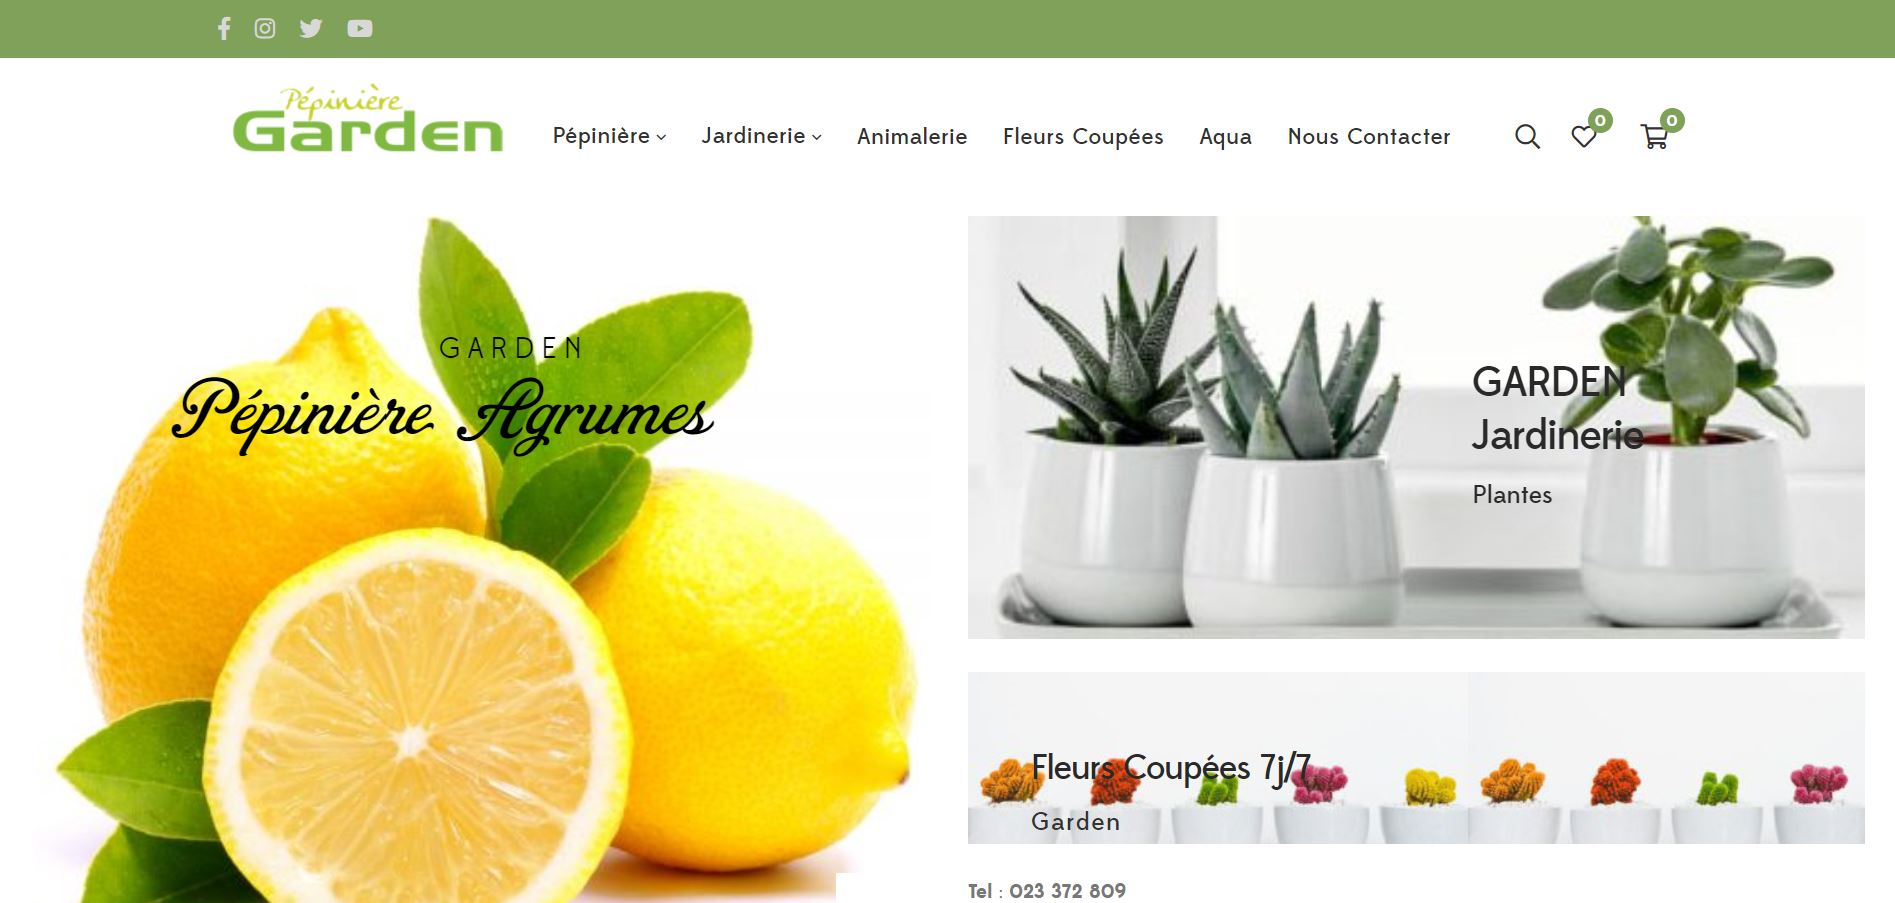
\includegraphics[width=1\textwidth]{Capture1}
  		\caption{La page d'accueil de la plateforme Garden Algerie}
		\end{figure}
		\vskip1cm
		\begin{figure}[h]
  		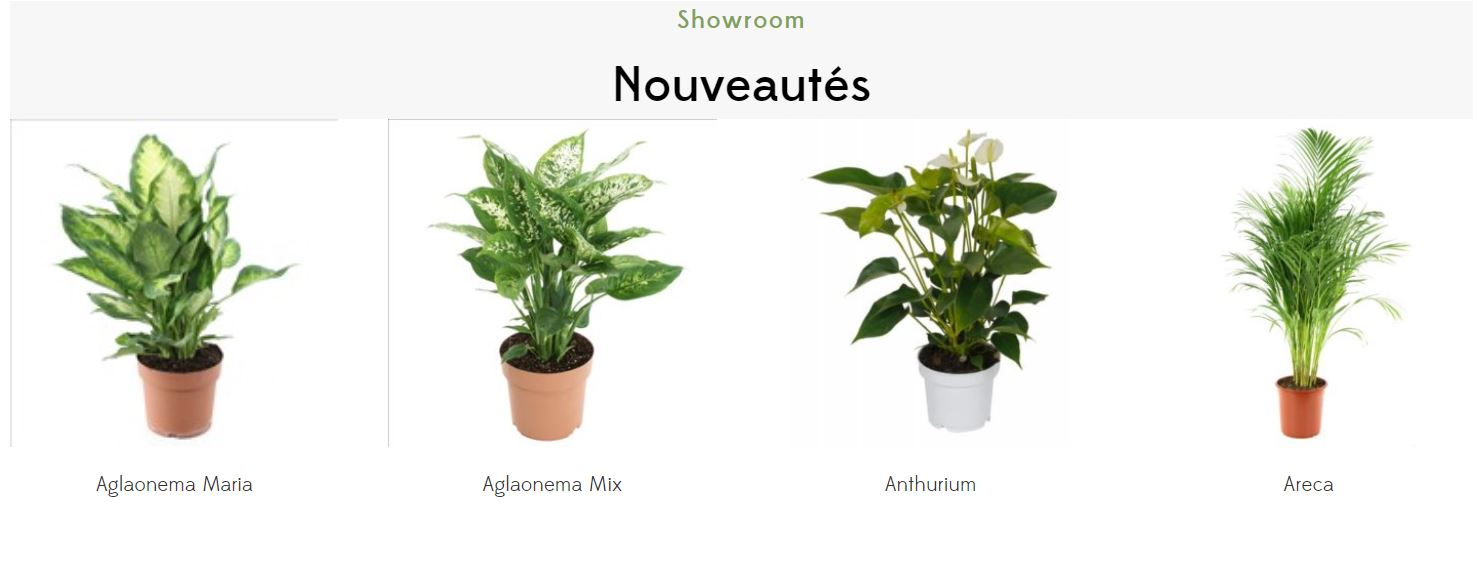
\includegraphics[width=1\textwidth]{Capture2}
  		\caption{La partie des nouveaux produits}
		\end{figure}
		
		\end{center}

\newpage

\subsubsection{Quelques critiques }
\begin{enumerate}
  \item On remarque dans cette plate-forme que le
design et plus vieux par rapport au grand
progrès dans le monde de design . De plus , on
peut dire qu'il est désorganisé , difficile à
utiliser.
  \item Difficulté de navigation : Ce sites web a des
structures de navigation complexes et difficiles
à comprendre, ce qui peut rendre la recherche
d'informations ou l'achat de produits plus
difficile pour les utilisateurs.
  \item Temps de chargement lent : il est aussi plus
lents à charger, ce qui peut frustrer les
utilisateurs et les inciter à quitter le site avant
même qu'il ne soit complètement chargé.
\item Manque de quelques fonctionnalités.
\end{enumerate}


\subsection{Analyse des besoins }
\subsubsection{Besoins fonctionnelles :}
\begin{enumerate}
  \item Gestion des stocks : Le magasin de plantes
doit être en mesure de gérer efficacement
son inventaire de plantes, de pots et d'autres
fournitures associées pour garantir la
disponibilité des produits en magasin.
  \item Gestion des clients : Le magasin doit pouvoir
gérer les informations de ses clients, telles
que les achats précédents, les préférences et
les coordonnées, pour offrir un service client
personnalisé.
  \item Suivi des commandes : Les clients peuvent
commander des plantes spécifiques ou des
quantités importantes pour des projets
spécifiques. Le magasin doit être en mesure de suivre les commandes et de s'assurer qu'elles
sont livrées dans les délais impartis.
\item Gestion des promotions : Le magasin doit être
en mesure de créer et de gérer des promotions et
des remises pour encourager les clients à acheter
davantage de plantes.
\end{enumerate}

\vskip2mm


* Ces besoins fonctionnels sont importants pour
garantir le bon fonctionnement et la réussite d'un
magasin de plantes.

\subsubsection{Besoins non fonctionnelles :}
\begin{enumerate}
  \item Sécurité : Le magasin doit être en mesure de
protéger les données personnelles de ses
clients, les transactions et les informations
commerciales confidentielles contre les
cyberattaques, les intrusions et les vols.
  \item Facilité d'utilisation : Le magasin doit être en
mesure de proposer une interface utilisateur
intuitive, facile à naviguer, facile à utiliser et
qui offre une expérience utilisateur agréable
pour ses clients.
  \itemÉvolutivité : Le magasin doit être en mesure
de s'adapter aux changements futurs de la
demande, de la concurrence, des
technologies et des réglementations pour
garantir sa pérennité et son développement.
\item Fiabilité : Le magasin doit être en mesure de
garantir la qualité de ses produits et services,
de respecter les délais de livraison et de
répondre rapidement et efficacement aux
demandes des clients pour maintenir leur
confiance et leur fidélité.
\item Éthique : Le magasin doit être en mesure de
respecter les normes éthiques,
environnementales et sociales pour assurer
une réputation positive et durable auprès de
ses clients et de la communauté.
\end{enumerate}

\vskip2mm
* Ces besoins non fonctionnels sont tout aussi
importants que les besoins fonctionnels pour
garantir le succès à long terme d'un magasin de
plantes.


\subsubsection{Diagramme de cas d’utilisation :}
Pour mieux comprendre le rôle de chaque acteur on utilise le
diagramme de cas d’utilisation dans lequel :

		\begin{itemize}
        \item[]
         $\bullet$  Le titre du diagramme est intitulé :site internet
    		\item[]
         $\bullet$  Dans notre cas on a 2 acteurs l’administrateur et le client .
         \item[]
         $\bullet$  L’administrateur a le droit de modifier le site ,d'ajouter une nouvelle catégorie, d'ajouter un nouveau produit et d'accepter une commande ou bien la refuser 
         \item[]
         $\bullet$  Pour le client on a 2 catégories en quelque sorte la première c’est pour la personne qui veut acheter directement en tant qu'un invité ( sans avoir à ouvrir un compte dans notre plateforme , il suffit juste  de saisir quelques données tels que leur nom et prénom, numéro de téléphone et son adresse ).dans la deuxième catégorie ,le client aura la capacité de se connecter et avoir un compte chez notre plateforme pour profiter de certaines offres. \\
         
         * Bien-sur dans les deux cas l’acteur restera le même (le client)

         $\bullet$  Pour chaque modifications les acteurs doivent être avec leurs comptes .
         
    		\end{itemize}





\newpage
		
		\begin{center}	
		{Site Internet}
  		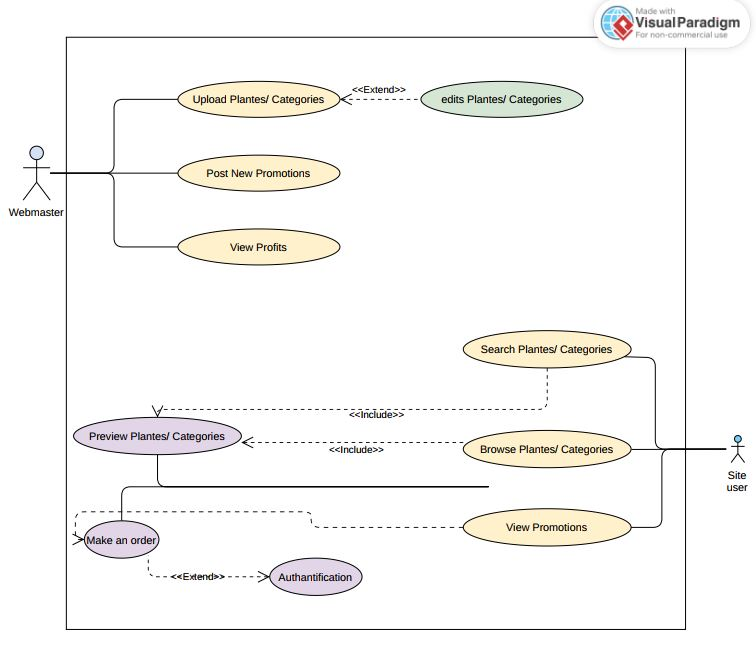
\includegraphics[width=1\textwidth]{Use Case Diagram}
		\end{center}
\vskip2mm
\subsection{Conclusion}
En conclusion, ce chapitre a permis de cerner les besoins et les attentes de notre client pour la plateforme de gestion de jardin de plantes, ainsi que les enjeux et les opportunités liés à ce projet. Nous avons identifié les fonctionnalités nécessaires pour répondre aux besoins des gestionnaires du jardin, ainsi que les critères de performance et de sécurité à prendre en compte dans le développement de la plateforme. Nous avons également analysé les solutions existantes et les critiques formulées à leur égard, afin de mieux comprendre les attentes des utilisateurs et les limites à dépasser. Dans le chapitre suivant, nous aborderons la conception de la plateforme en détaillant les choix de conception et les modèles retenus pour répondre aux besoins et aux enjeux identifiés.
\newpage


\section{CHAPITRE 02 : Conception}
{\fontsize{15}{20}\selectfont 
\subsection{Introduction}

\hspace{1cm} Le deuxième chapitre de notre rapport est consacré à la conception de notre plateforme de gestion de jardin de plantes de Mr \textbf OUCHEN AHCENE. Après avoir identifié les besoins spécifiques de notre client et les fonctionnalités clés de notre plateforme dans le premier chapitre, nous allons maintenant nous concentrer sur la modélisation de notre solution. Cette étape est cruciale pour assurer une implémentation efficace et une architecture cohérente de la plateforme. Dans ce chapitre, nous allons présenter les différentes étapes de la conception de notre plateforme, notamment la création de différents diagrammes de séquence et de classe, ainsi que la modélisation de la base de données relationnelle. Nous expliquerons également les choix de conception que nous avons faits pour répondre aux besoins spécifiques du jardin .

\subsection{Diagrammes de séquence}
\hspace{1cm} Les diagrammes de séquences sont des outils de modélisation qui permettent de décrire les interactions entre les différents acteurs et les objets d'un système. Ils sont particulièrement utiles pour représenter des processus complexes tels que l'authentification d'un utilisateur, l'ajout d'un produit ou l'achat d'un produit dans le cadre de notre projet.

Dans cette partie, nous allons nous concentrer sur trois diagrammes de séquences clés de votre projet : le premier pour l'authentification, le deuxième pour l'ajout d'un produit et le troisième pour l'achat d'un produit. Nous allons examiner chaque diagramme en détail, en expliquant les différentes étapes du processus et en soulignant les interactions entre les différents acteurs et objets du système.

En examinant ces diagrammes de séquences, nous pourrons mieux comprendre comment notre système fonctionne et comment les différents acteurs interagissent avec lui pour atteindre leurs objectifs.

\newpage
\subsubsection{Authentification}
\vskip2cm
		\begin{center}
  		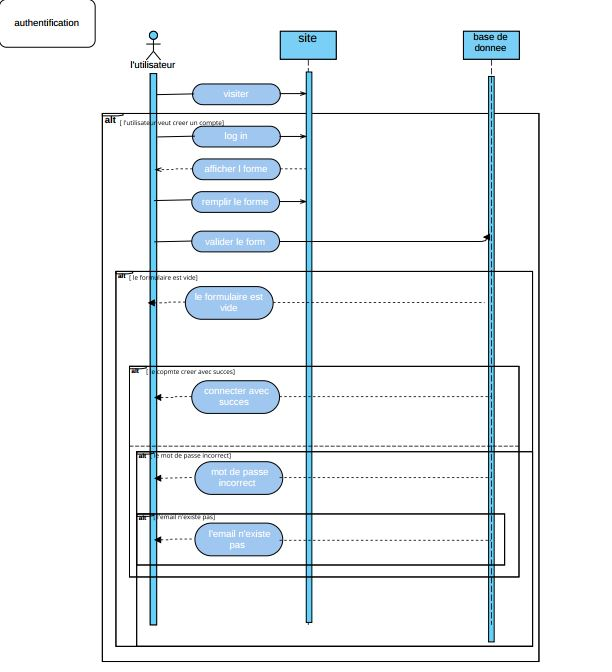
\includegraphics[width=1\textwidth]{Authentification}
		\end{center}

\newpage
\subsubsection{Ajouter Un produit }
\vskip2cm
		\begin{center}
  		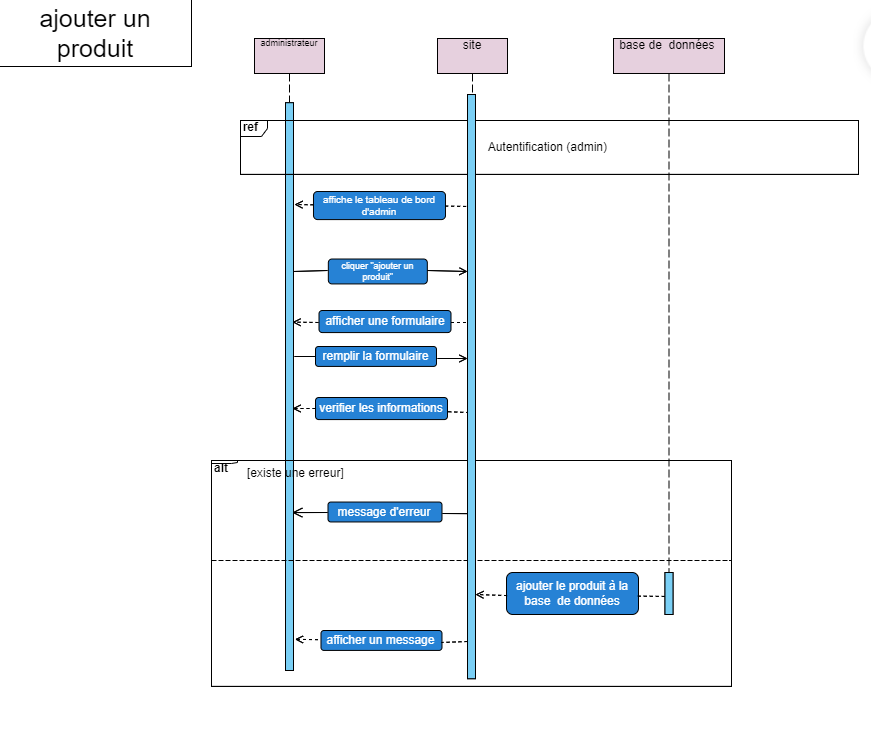
\includegraphics[width=1\textwidth]{Ajouter Un produit}
		\end{center}
		
		\newpage
\subsubsection{Acheter Un produit }
\vskip2cm
		\begin{center}
  		\includegraphics[width=1\textwidth]{Acheter Un produit}
		\end{center}
		
\newpage


\subsection{Diagramme de classe}
\hspace{1cm} Le diagramme de classe est un outil de modélisation essentiel pour la conception de systèmes orientés objet. Il représente les classes, les attributs, les méthodes et les relations entre les objets d'un système. Le but de cette partie est donc de concevoir le diagramme de classe pour notre système en prenant en compte les besoins des clients et les fonctionnalités du système. La conception du diagramme de classe est une étape importante dans le développement du système, car elle permet de définir l'architecture globale du système et de planifier la mise en œuvre.\\
\hspace{1cm} Il est donc crucial de bien comprendre les besoins des clients et les fonctionnalités du système pour pouvoir concevoir un diagramme de classe clair et précis. Nous examinerons également les rôles et les autorisations des différents acteurs du système, tels que les clients et les responsables, afin de garantir que les fonctions et les interactions du système sont bien définies.

\begin{itemize}
        \item[]
         $\bullet$ Les clients ont l'accès à la fonctionnalité d'achat des produits dans notre système. Ils pourront naviguer sur le site, rechercher des produits, ajouter des produits à leur panier, passer des commandes et payer en utilisant les options de paiement disponibles. Les clients auront également la possibilité de consulter leur historique de commande et leur profil personnel pour mettre à jour leurs informations.
    		\item[]
         $\bullet$  Les responsables ont un accès plus avancé au système par rapport aux clients. Ils pourront ajouter, modifier et supprimer des produits, gérer les commandes des clients et gérer les informations de livraison. Ils pourront également visualiser les rapports de vente et les statistiques du système pour prendre des décisions commerciales éclairées. Les responsables auront également la possibilité de consulter et de modifier leur profil personnel.
                
    		\end{itemize}
\newpage
		\begin{center}
  		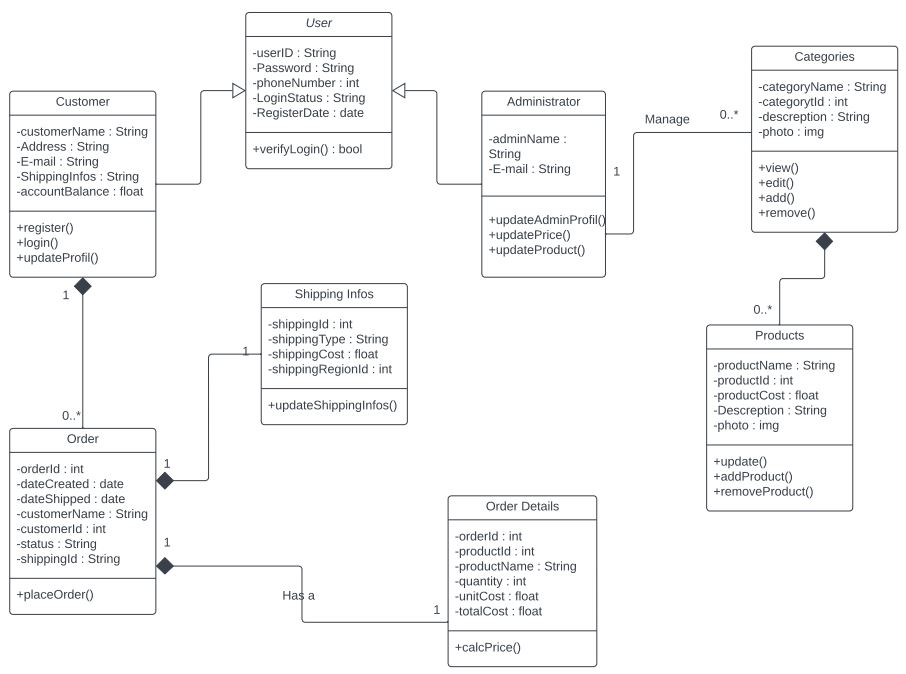
\includegraphics[width=1\textwidth]{Class diagramm}
		\end{center}


\subsection{Conclusion}

\hspace{1cm} En conclusion, le chapitre 02 a permis de détailler la conception de notre plateforme à travers l'élaboration de différents diagrammes de séquences qui ont permis de représenter les différentes fonctionnalités de l'application. Nous avons également présenté les diagrammes de classes qui ont permis de modéliser les différentes entités du système ainsi que leurs relations. Ces différents diagrammes ont permis de clarifier l'architecture de l'application et de mieux comprendre le fonctionnement de chaque module. Dans le prochain chapitre, nous allons aborder la partie implémentation en nous basant sur la conception réalisée dans ce chapitre.

}


\newpage
\section{CHAPITRE 03 : Réalisation}
{\fontsize{15}{20}\selectfont 
\subsection{Introduction}

\hspace{1cm} Le site PlantEz est un site web qui est réalisé par une équipe d’étudiants de l’école supérieure de
sciences et technologies d’informatique et numérique–Bejaia dans le cadre d’un projet
pluridisciplinaire de fin de cycle préparatoire,destiné aux clients et au propriétaire de la pininiere
fleuriste . Notre application web destinée à deux types d’utilisateurs (Admin, clients) afin de régler
les différents problèmes et aussi pour faciliter la tâche aux clients pour un service mieux et
confortable.

Dans ce chapitre on va représenter la partie technique et concrète de notre projet, où nous
allons détailler les étapes de développement, en partant de la conception de l’interface utilisateur
jusqu’à l’implémentation des fonctionnalités les plus avancées. Ce chapitre expose les choix
techniques que nous avons effectués pour répondre aux besoins et aux attentes des utilisateurs,
Nous allons également décrire les différentes interfaces formant notre site et les tests que nous
avons effectués pour garantir son bon fonctionnement.

\subsection{Outils de développement}
{\fontsize{15}{20}\selectfont
\begin{enumerate}
  	\item Design :
  		\begin{itemize}
        \item[] $\bullet$ Figma : 
        C'est un outil très populaire pour la conception d’interfaces utilisateur (UI) et
la création de prototypes. Il permet aux designers de travailler de manière collaborative
et en temps réel sur des projets de design. Il offre egalement des fonctionnalités telles que
la création de maquettes de conception, la personnalisation des couleurs et des polices,
ainsi que la création d’animations et de transitions. Grâce à sa facilité d’utilisation et à
sa grande flexibilité.
    		\item[] $\bullet$ Photoshop
    		\item[] $\bullet$ https://www.canva.com
    		\item[] $\bullet$ illustrator
    		    
    		\end{itemize}
    		\newpage
    		\begin{figure}
    		\centering
		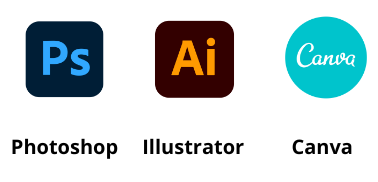
\includegraphics[width=10cm]{logos}
		\end{figure} 
    	\item Front-end : Nous avons utilisé les technologies suivantes : 
 		\begin{itemize}
        \item[] $\bullet$ Html : c’est le langage de balisage standard pour la création de pages web. Il permet dedéfinir la
structure de base du site y compris les titres, les paragraphes, les images,
les liens, les formulaires, etc.
    		\item[] $\bullet$ Css : C’est un langage qui permet de définir la présentation d’une page web, notamment
les couleurs, les polices, les mises en page, les bordures, les arrière-plans, etc. Il
permet de personnaliser l’apparence de site web pour le rendre plus attrayant.
    		\item[] $\bullet$ Javascript : c’est un langage de programmation qui permet d’ajouter des fonctionnalités inter-
actives à un site web. Par exemple, Nous pouvons utiliser JavaScript pour créer des
animations, des menus déroulants, des pop-ups, des carrousels d’images, etc. 
\item[] $\bullet$ Bootstrap

Car : 
\begin{itemize}
    \item Faciliter de réalisation de liens d’un serveur vers un
autre
    \item Le texte HTML peut être écrit avec un éditeur standard.
    \item On peut réaliser assez facilement un serveur.
    \item Le principal avantage de CSS est que le style est appliqué de manière cohérente sur une variétè de sites.
    \item CSS applique automatiquement les styles requis.
    \item Il a le pouvoir de se repositionner. Cela nous aide `a
d´eterminer les changements dans la position des éléments
Web présents sur la page.



\item Le plus grand avantage de JavaScript étant sa capacité
à prendre en charge tous les navigateurs modernes et `a
produire un résultat équivalent.
\item Il existe de nombreux projets open source qui fournissent une aide utile à l’ajout de JavaScript par le développeur.
\item Il existe de nombreux cours disponibles dans le domaine
de Java-Script.
\end{itemize}  
\end{itemize}

		\begin{figure}[h]
		\centering
		
\includegraphics[width=10cm]{html-css-js}
		\end{figure} 
		
 	\item Back-end : 
 		\begin{itemize}
        \item[] $\bullet$ Node js : c’est un environnement d’exécution JavaScript côté serveur qui permet de dévelop-
per des applications rapides et évolutives. Il permet également aux développeurs de
travailler avec des langages familiers, tels que JavaScript et JSON.
    		\item[] $\bullet$ Express : c’est un framework d’application Web pour Node.js. Il fournit une structure robuste
pour les applications Web et les API, ainsi que des fonctionnalités telles que le
routage, les middlewares et les gestionnaires d’erreurs.
    		\item[] $\bullet$ EJS : c’ est un langage de modèle simple qui vous permet de générer un balisage HTML
avec du JavaScript simple. Aucune religiosité sur la façon d’organiser les choses.
Pas de réinvention de l’itération et du flux de contrôle. C’est tout simplement du
JavaScript. (EJS p. d.)
    		\item[] $\bullet$ Body-parser : il sert à analysez les corps de requête entrants dans un middleware avant vos ges-
tionnaires, disponibles sous la req.bodypropriété. (Body-parser p. d.)
    		\item[] $\bullet$ Morgan pachage : Intergiciel de journalisation des requêtes HTTP pour node.js (Morgan p. d.)
             
    		\end{itemize} 
    		\newpage
    	\item Base de données : 
 		\begin{itemize}
        \item[] $\bullet$ Mongo DB Atlas : MongoDB Atlas est un service de base de données multi-cloud par les mêmes per-
sonnes qui ont construit MongoDB. Atlas simplifie le déploiement et la gestion de
vos bases de données tout en offrant la polyvalence dont vous avez besoin pour créer
des applications globales résilientes et performantes sur les fournisseurs de cloud de
votre choix. (Mongo DB Atlas p. d.)
    		\item[] $\bullet$ Mongoose : c’est une bibliothèque ODM (Object Data Modeling) pour MongoDB et Node.js. Il
gère les relations entre les données, fournit une validation de schéma et est utilisé
pour traduire entre les objets dans le code et la représentation de ces objets dans
MongoDB. (Mongoose p. d.)     
    		\end{itemize} 
    		\begin{figure}[h]
		\centering
		
\includegraphics[width=10cm]{MERN-logo}
		\end{figure}
		
		
    	\item Editeur de codes : \\
 		Des éditeurs de code comme VS Code, Nous permettons de créer et d’éditer du
code HTML, CSS et JavaScript plus rapidement et plus efficacement. Ces outils sont
équipés de fonctionnalités pratiques telles que la coloration syntaxique, la compélation automatique, la prévisualisation en direct et la gestion de versions.
	
		
		
	\item Communication : 
 		\begin{itemize}
        \item[] $\bullet$ Github desktop : car c’est un outil de gestion de version qui facilite la
collaboration en groupe dans un projet . Il permet aux membres du groupes de travailler
ensemble sur le même code source de suivre les modifications apportées
    		\item[] $\bullet$ Email
    		\item[] $\bullet$ Messenger
    		\item[] $\bullet$ Discord
    		\item[] $\bullet$ Drive     
    		\end{itemize}
    		\begin{figure}[h]
		\centering
		
\includegraphics[width=5cm]{git-disc}
		\end{figure}
  	\item La diapo de présentation : 
  	 	\begin{itemize}
        \item[] $\bullet$ https://www.canva.com
        \item[] $\bullet$ Photoshop
        \item[] $\bullet$ Figma     
    		\end{itemize} 
    		\begin{figure}[h]
		\centering
		
\includegraphics[width=5cm]{figma-logo-0}
		\end{figure}
	\item Le rapport et le cahier de charge :	
		\begin{itemize}
        \item[] $\bullet$ Latex
        \end{itemize}
        \begin{figure}[h]
		\centering
		
\includegraphics[width=5cm]{LaTeX_logo.svg}
		\end{figure}
\end{enumerate}
}

\newpage


\subsection{Présentation de l’application}
\subsubsection{Présentation du Nom de la plateforme :}
	\begin{figure}[h]
	\centering
	
\includegraphics[width=12cm]{nom}
	\end{figure}
\subsubsection{Présentation du logo :}

		\begin{center}
  		
\includegraphics[width=5cm]{LOGO last version}
		\end{center}
		
		\begin{center}
  		\fbox{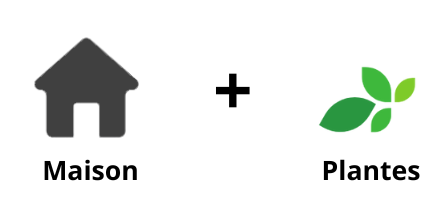
\includegraphics[width=10cm]{presentation}}
		\end{center}
		
\begin{figure}[h]
  \begin{minipage}{0.48\textwidth}
    \centering
    
\includegraphics[width=5cm]{2}
    
    
  \end{minipage}
  \hfill
  \begin{minipage}{0.48\textwidth}
    \centering
    
\includegraphics[width=5cm]{3.png}
    
    
  \end{minipage}
\end{figure}
		
\vskip1mm
\newpage
		\begin{itemize}
		\item[] $\bullet$ Quelques mocups pour la présentaion du 				LOGO
		\begin{center}
  		
\includegraphics[width=11cm]{mocup3}
		\end{center}
		\begin{center}
  		\includegraphics[width=11cm]{mocup2}
		\end{center}
		\begin{center}
  		\includegraphics[width=11cm]{mocup1}
		\end{center}
		\end{itemize}
		
\newpage

\begin{minipage}{0.48\textwidth}
		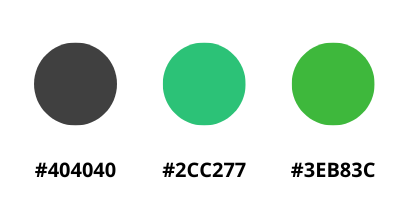
\includegraphics[width=6cm]{colors}
\end{minipage}
\begin{minipage}{0.48\textwidth}
		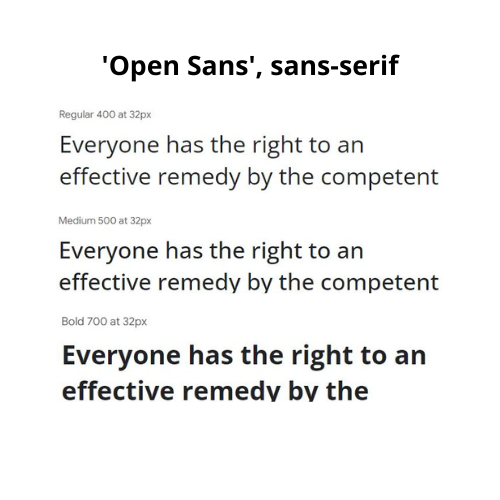
\includegraphics[width=10cm]{fonts}
\end{minipage}



\subsubsection{Présentation des interfaces}
\begin{enumerate}
  	\item Interfaces client :
  	\begin{itemize}
  	\item Page d'accueil :
  	Elle représente la première page visible pour les deux parties prenantes , Cette page est
dotée d’une barre de navigation qui contient des liens hypertexte menant aux différentes
fonctionnalités du site.
		\begin{figure}[h]
		\centering
  		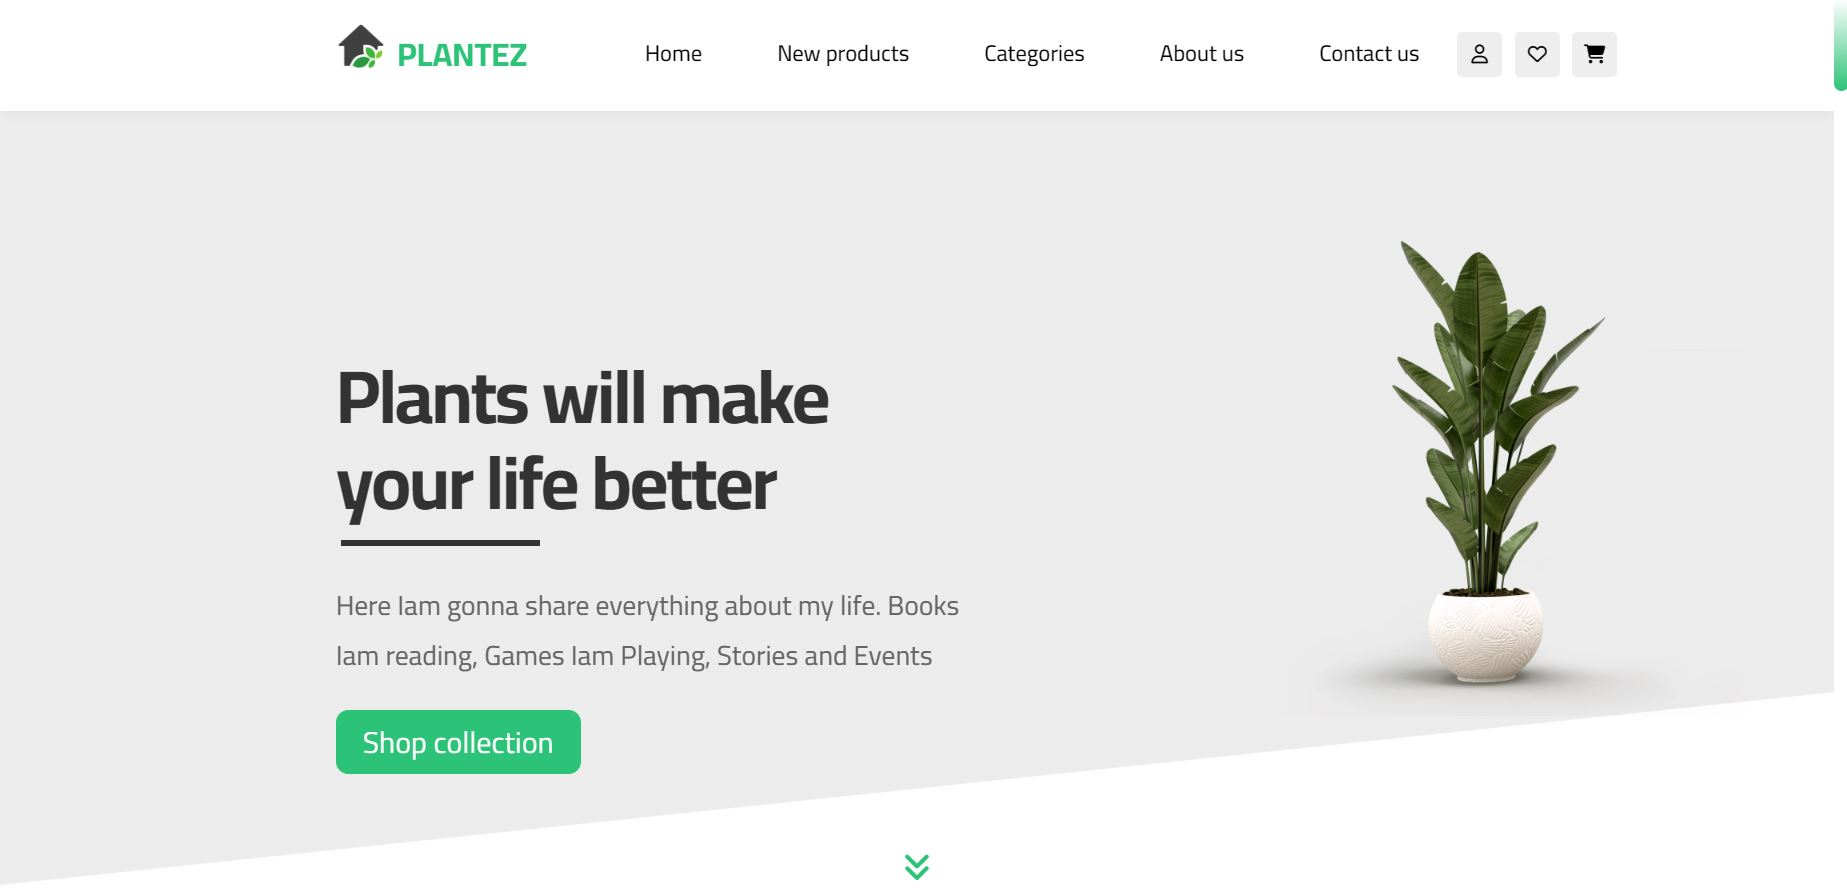
\includegraphics[width=15cm]{home}
  		\caption{La page d'accueil de la plateforme PLANTEZ}
		\end{figure}
		
		\item on a ensuite une exposition des offres existant dans une période donnée
  	
		\begin{figure}[h]
		\centering
  		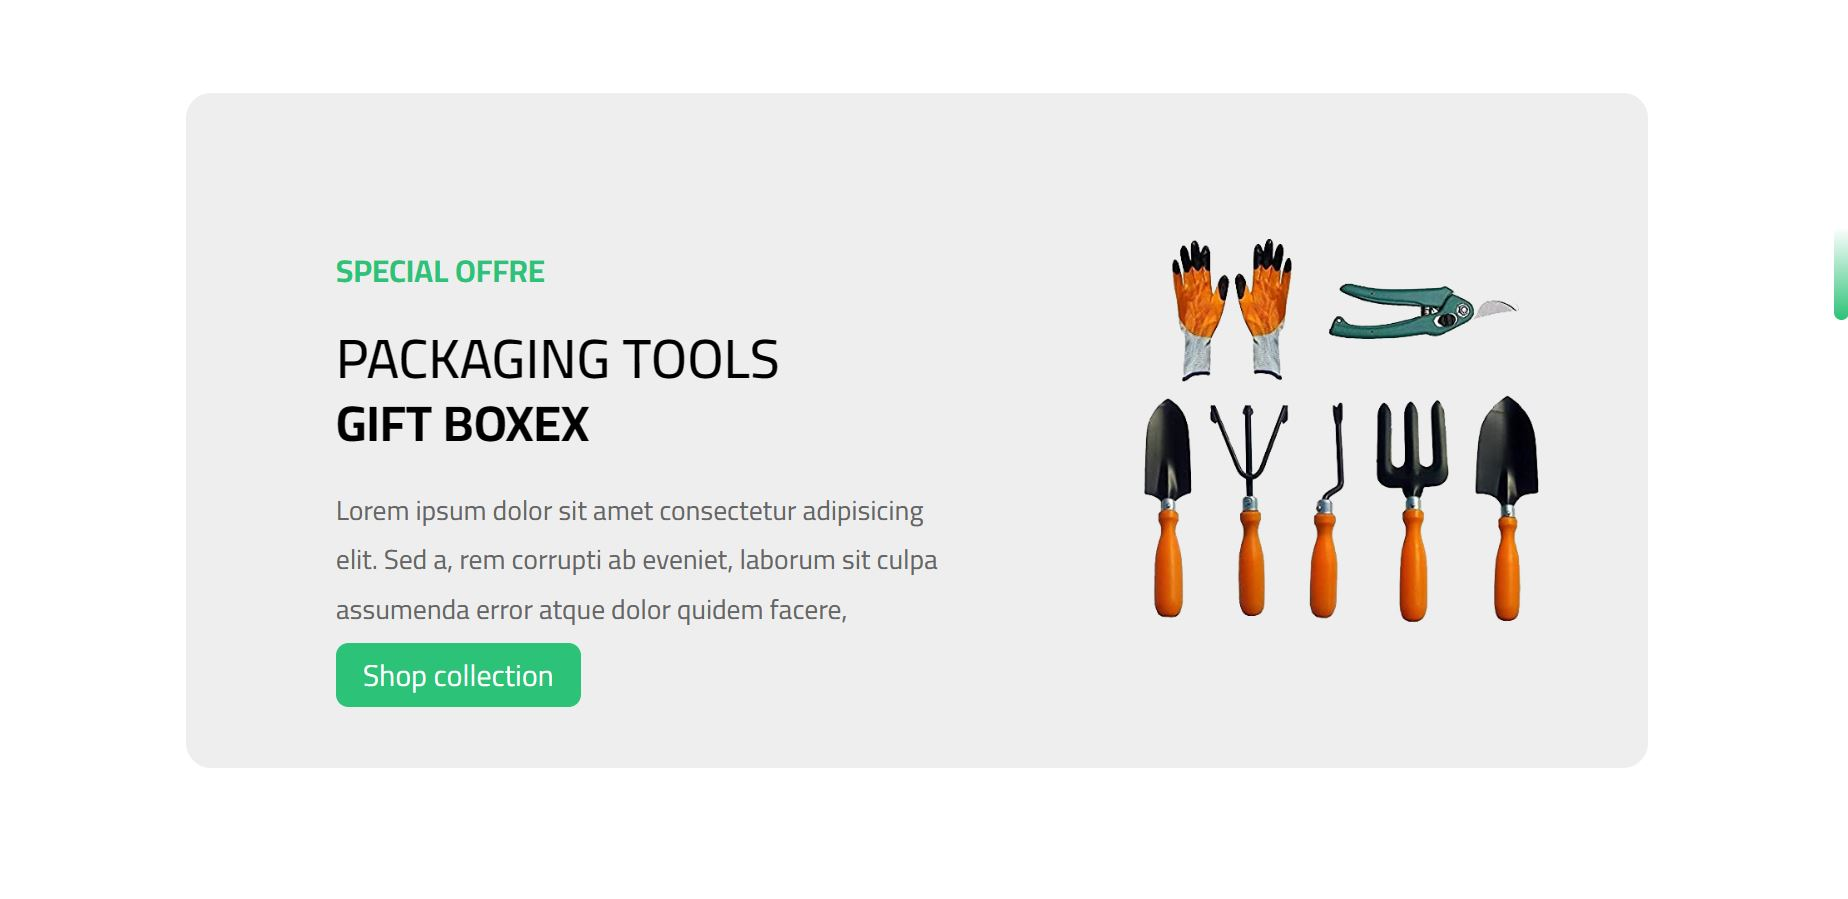
\includegraphics[width=15cm]{offre}
  		\caption{Offres existant dans une période donnée}
		\end{figure}
		
		\item En outre, la page d’accueil comprend une zone dédiée aux quelques categories qui seront
proposées, accompagnée d’un lien permettant d’accéder aux produits de chaque category
  	
		\begin{figure}[h]
		\centering
  		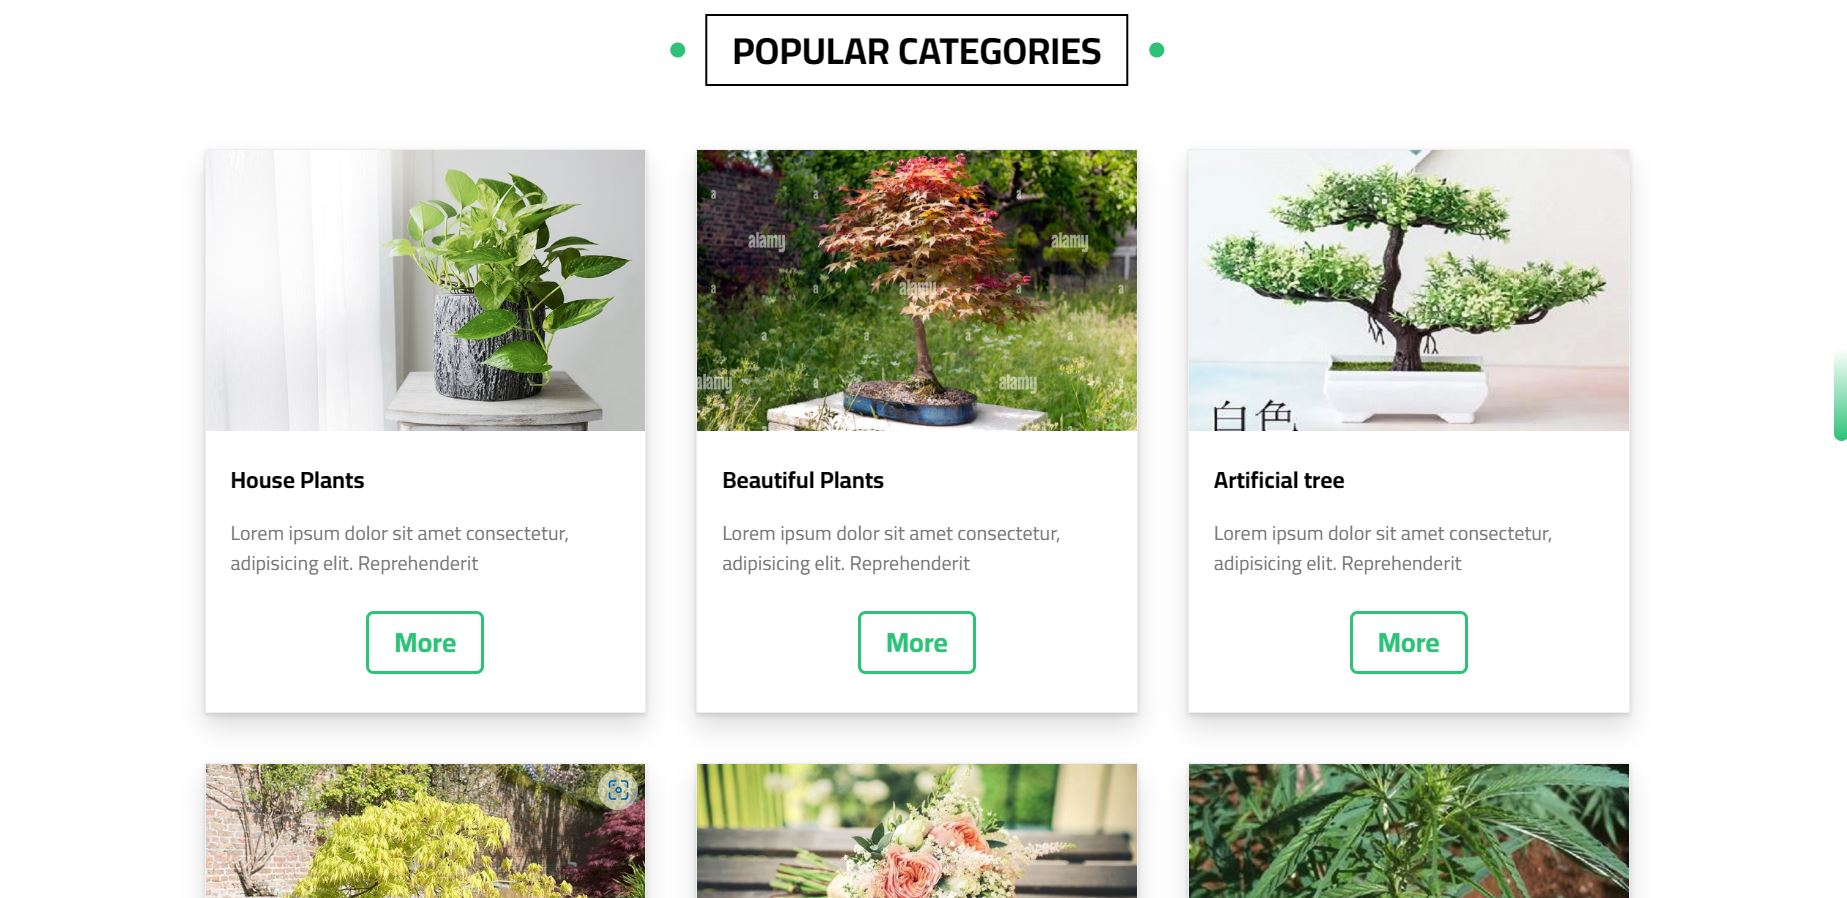
\includegraphics[width=15cm]{categories}
  		\caption{Catégories proposées}
		\end{figure}
		
  	\end{itemize}
  	
  	
  	
  	\begin{itemize}
  	\item Page de catégories : 
  	Au dessous de cette zone , il y a un button qui conduit à la page de \textbf Categories ; qui contient la
listes des categories existantes dans notre site :
\newpage
		\begin{minipage}{0.48\textwidth}
		
\includegraphics[width=6cm]{plus-cat}
		\end{minipage}
		\begin{minipage}{0.48\textwidth}
		
\includegraphics[width=6cm]{plus-cat-hover}
		\end{minipage}
		
		\vskip1cm
		\item Et chaque category contient une liste des produits :
  	
		\begin{figure}[h]
		\centering
  		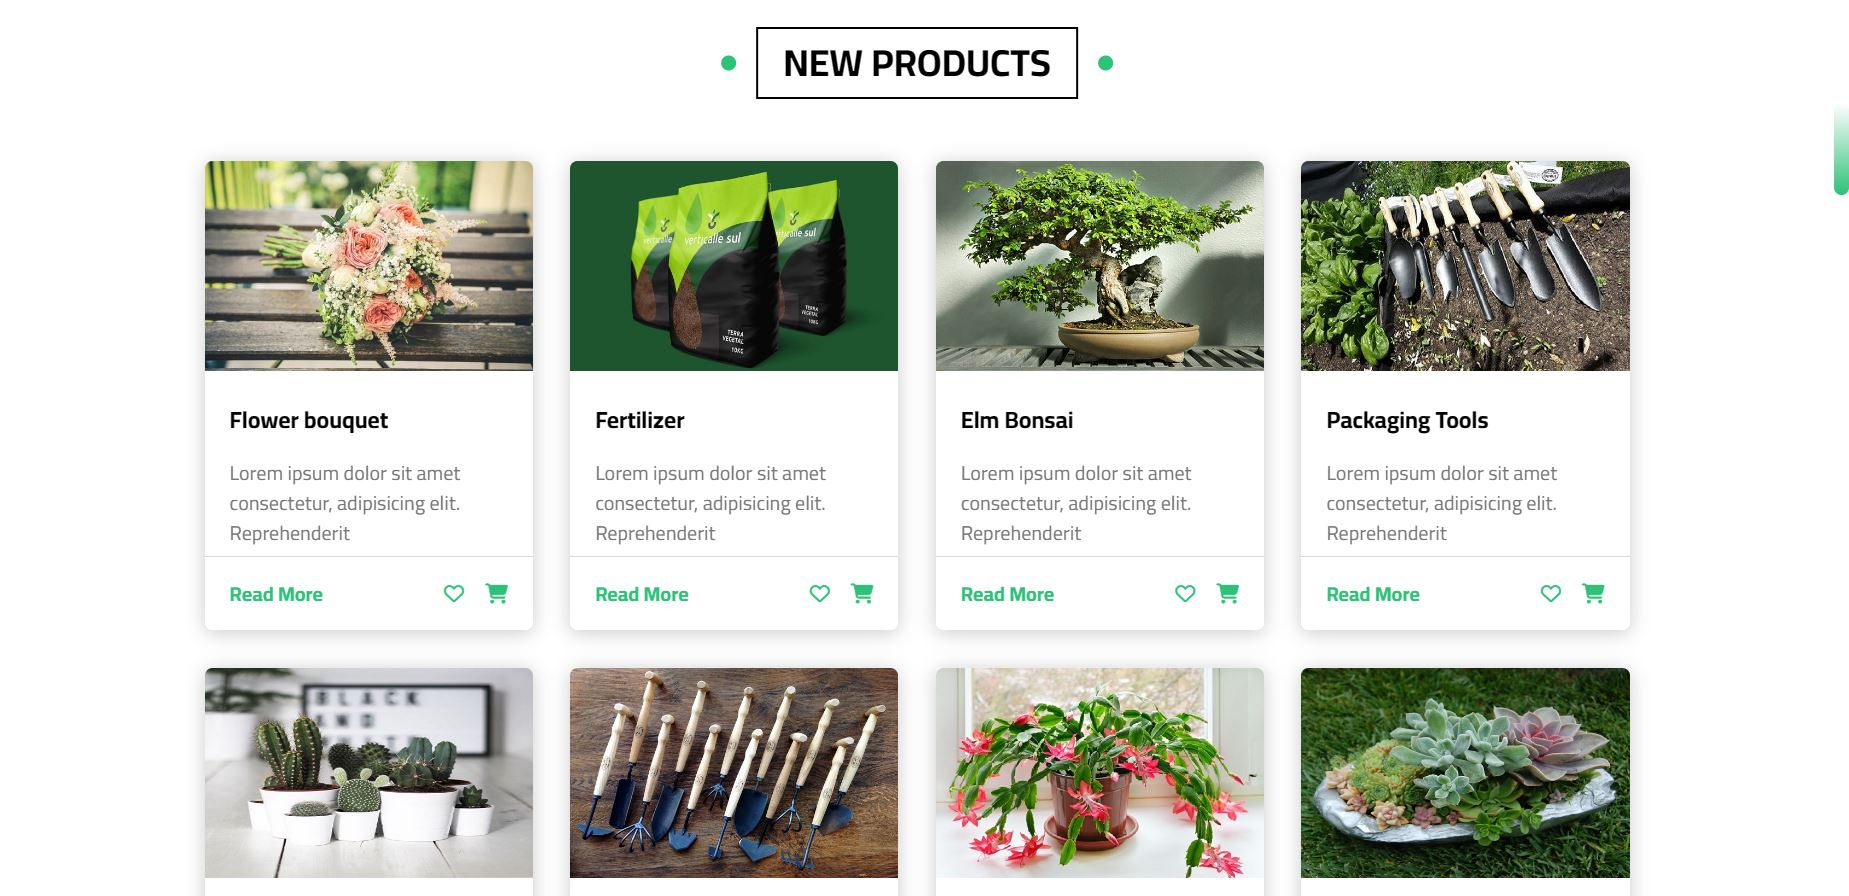
\includegraphics[width=15cm]{prod}
  		\caption{Liste des produits}
		\end{figure}
		
		\vskip1cm
		\item Lorsqu’on accède à l’un des produits existants au niveau de la page des produits , le client va être
rediriger vers une page qui contient des informations générales et plus detaillés ,
  	
		\begin{figure}[h]
		\centering
  		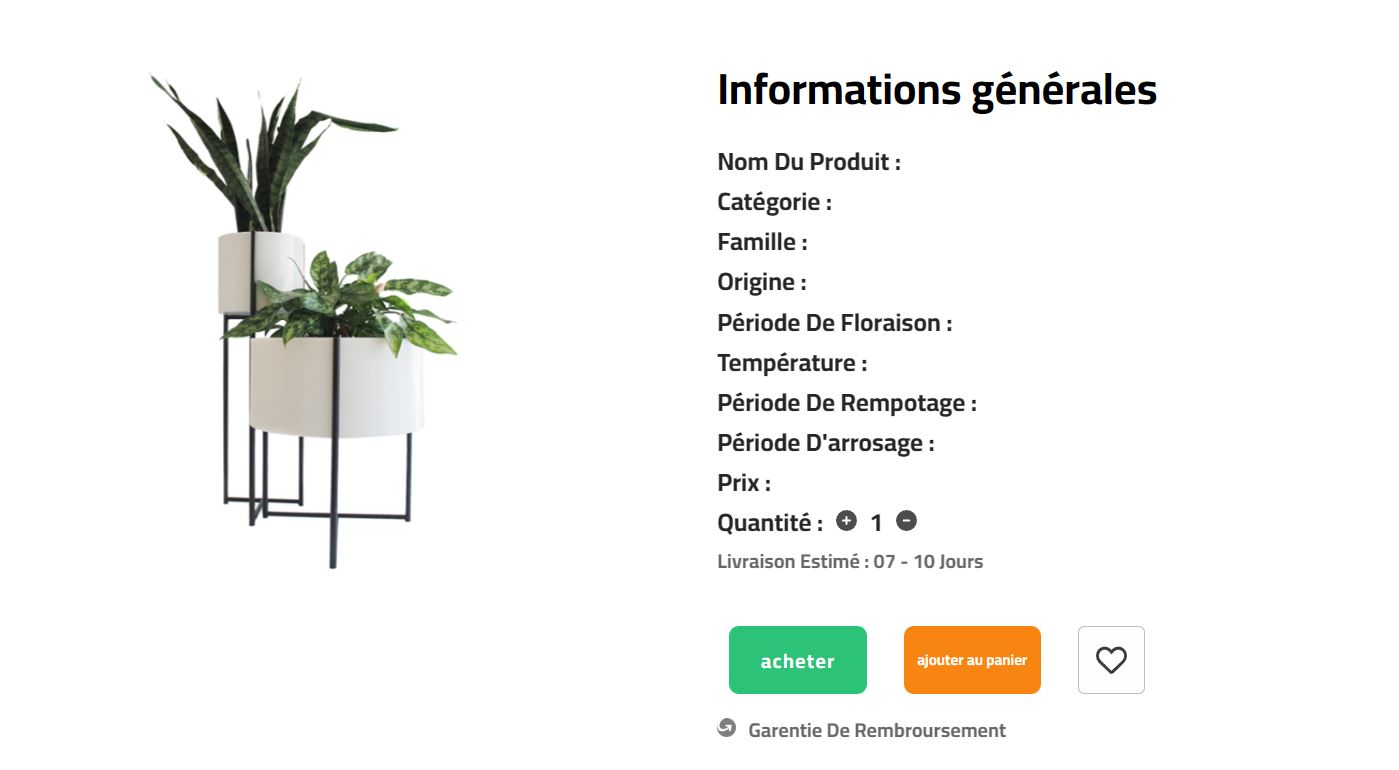
\includegraphics[width=12cm]{products}
  		\caption{Informations du produit}
		\end{figure}
		
		\item Ensuite , le client détermine la quantité qu’il veut acheter puis cliquer sur acheter .
		\item La figure ci-dessous représente un formulaire qui contient le prix général de ce produit .
		\begin{figure}[h]
		\centering
  		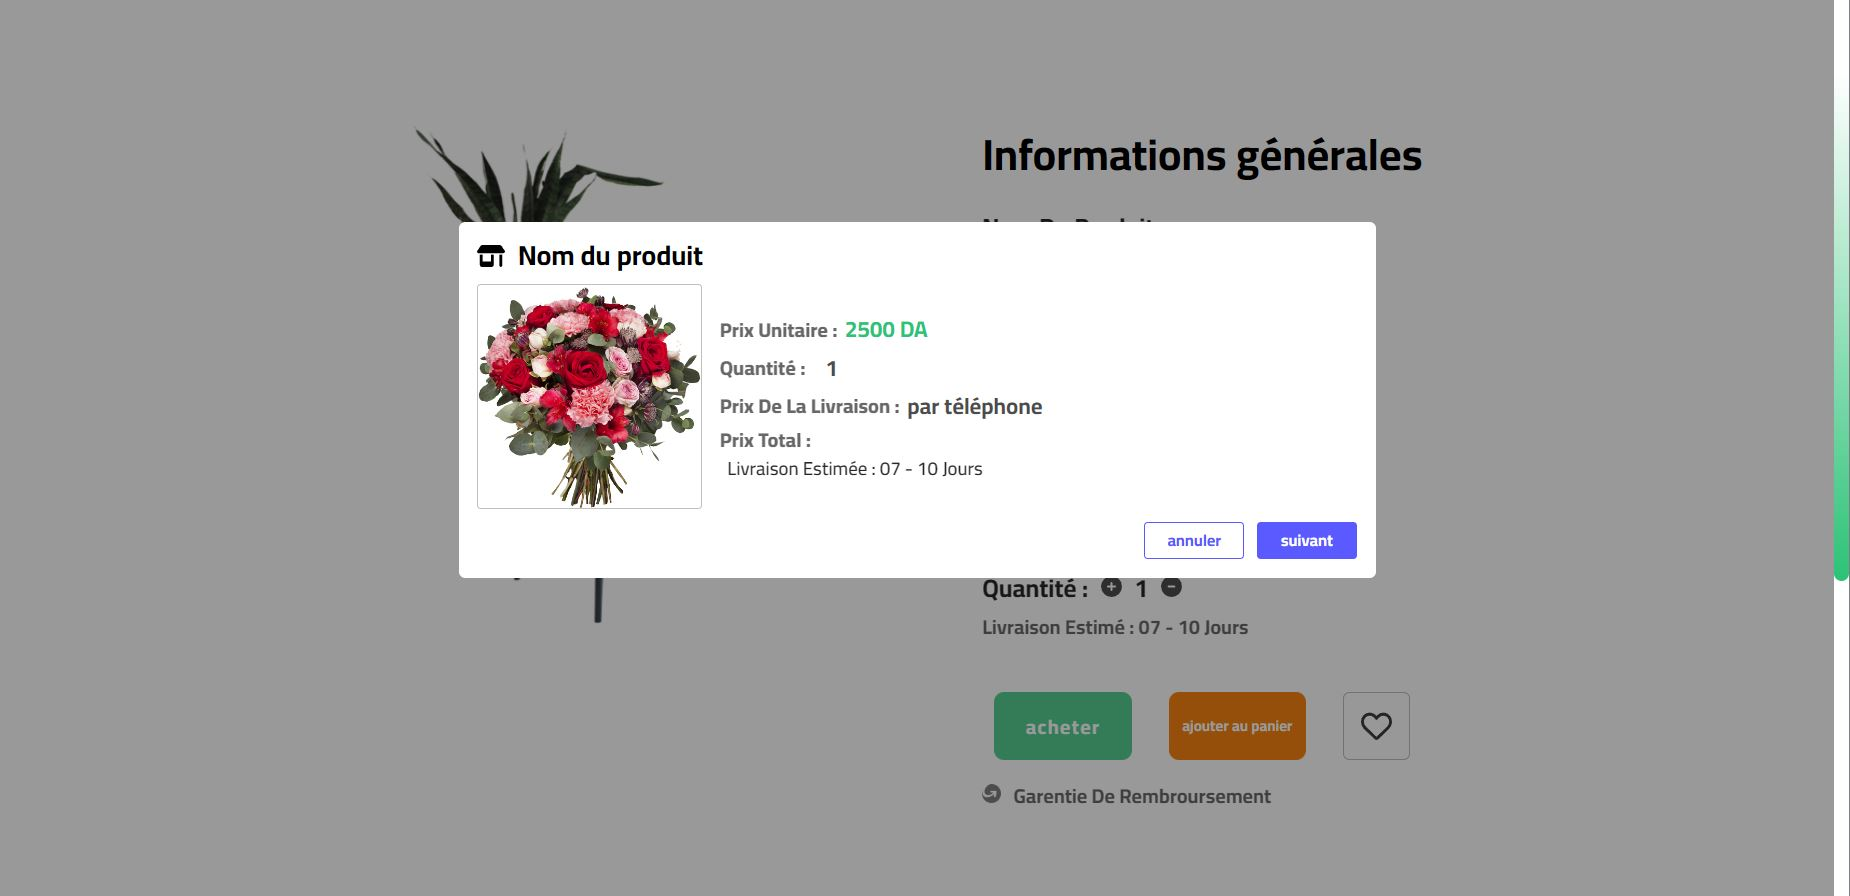
\includegraphics[width=12cm]{nomduproduit}
  		\caption{Informations du produit}
		\end{figure}
		
		\item En cas de réponse positive , un formulaire supplémentaire apparaitra, pour lui permettre de
spécifier ces informations personnelles , tels que le nom ,le prénom, le numéro de téléphone et l'adresse .
\begin{figure}[h]
		\centering
  		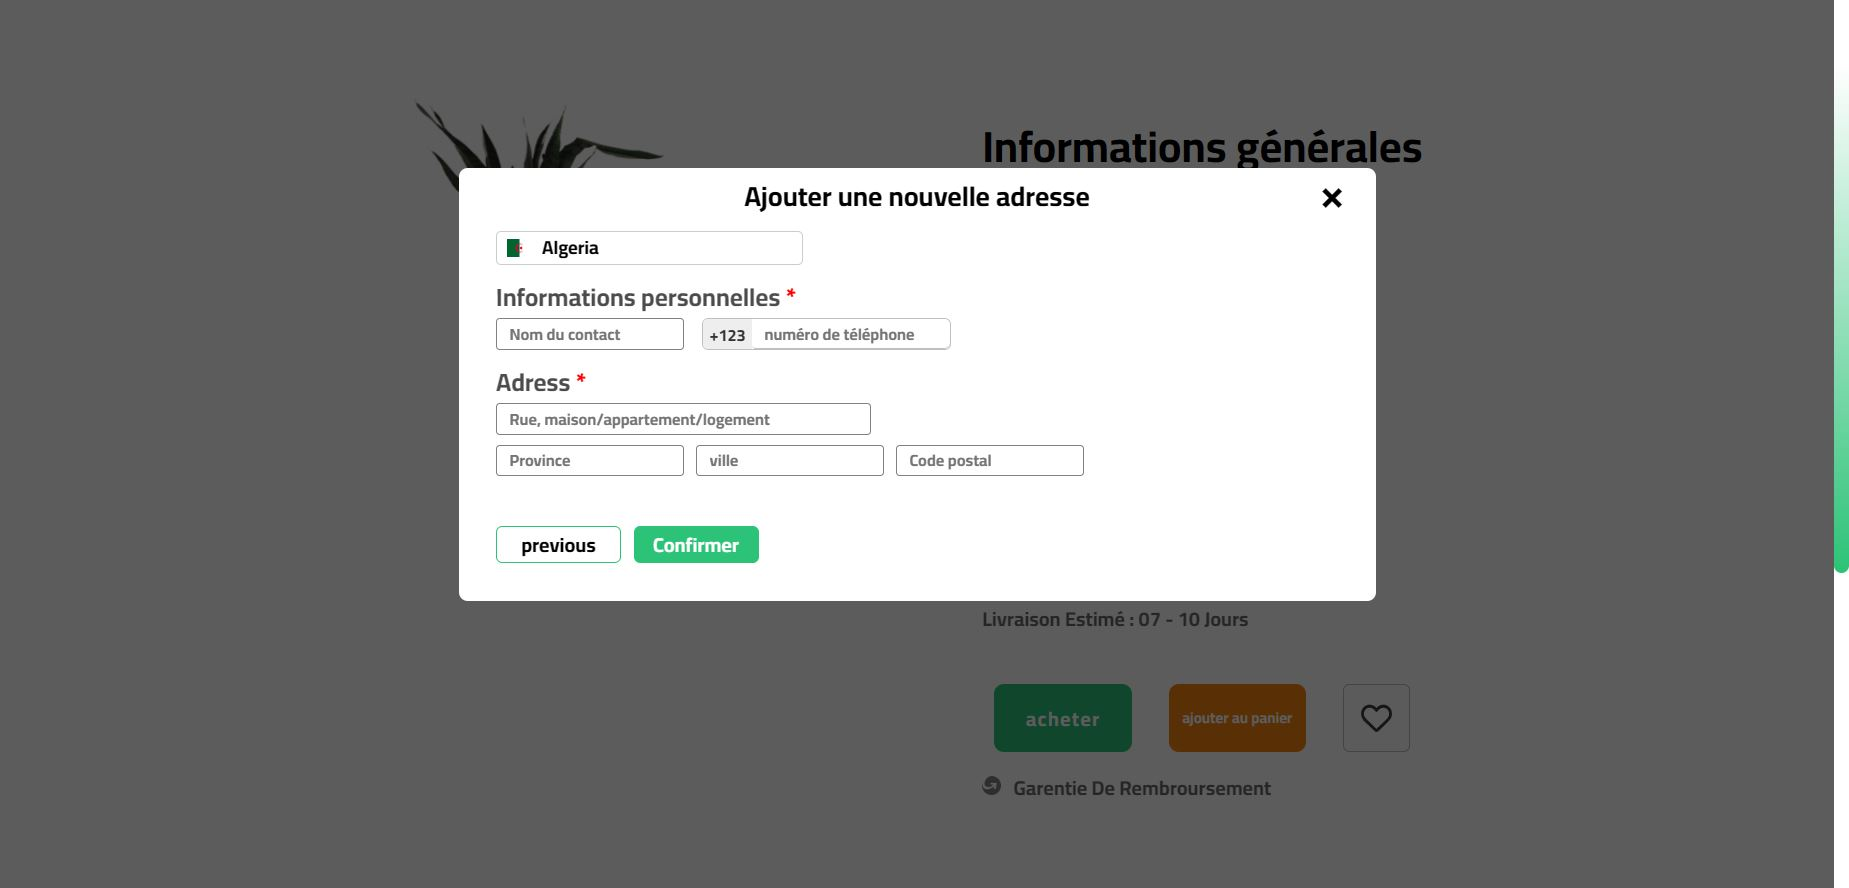
\includegraphics[width=12cm]{supp}
		\end{figure}
		
		\item Après avoir saisi toutes les données nécessaires, le client pourra cliquer sur le bouton ‘confirmer’
pour finaliser la demande ou bien sur le boutton 'annuler' pour l’abondonner .
\newpage
		
		\item Panier et favoris :
		Pour ajouter le produit aux panier ou bien aux favoris, il faut que vous soyez déjà inscrits pour voir
plus de détails.
Alors si vous êtes déjà inscrit connectez-vous directement sinon créez un compte ou connectez-vous
via Google pour faciliter la connexion.		
		
		\begin{figure}[h]
		\centering
  		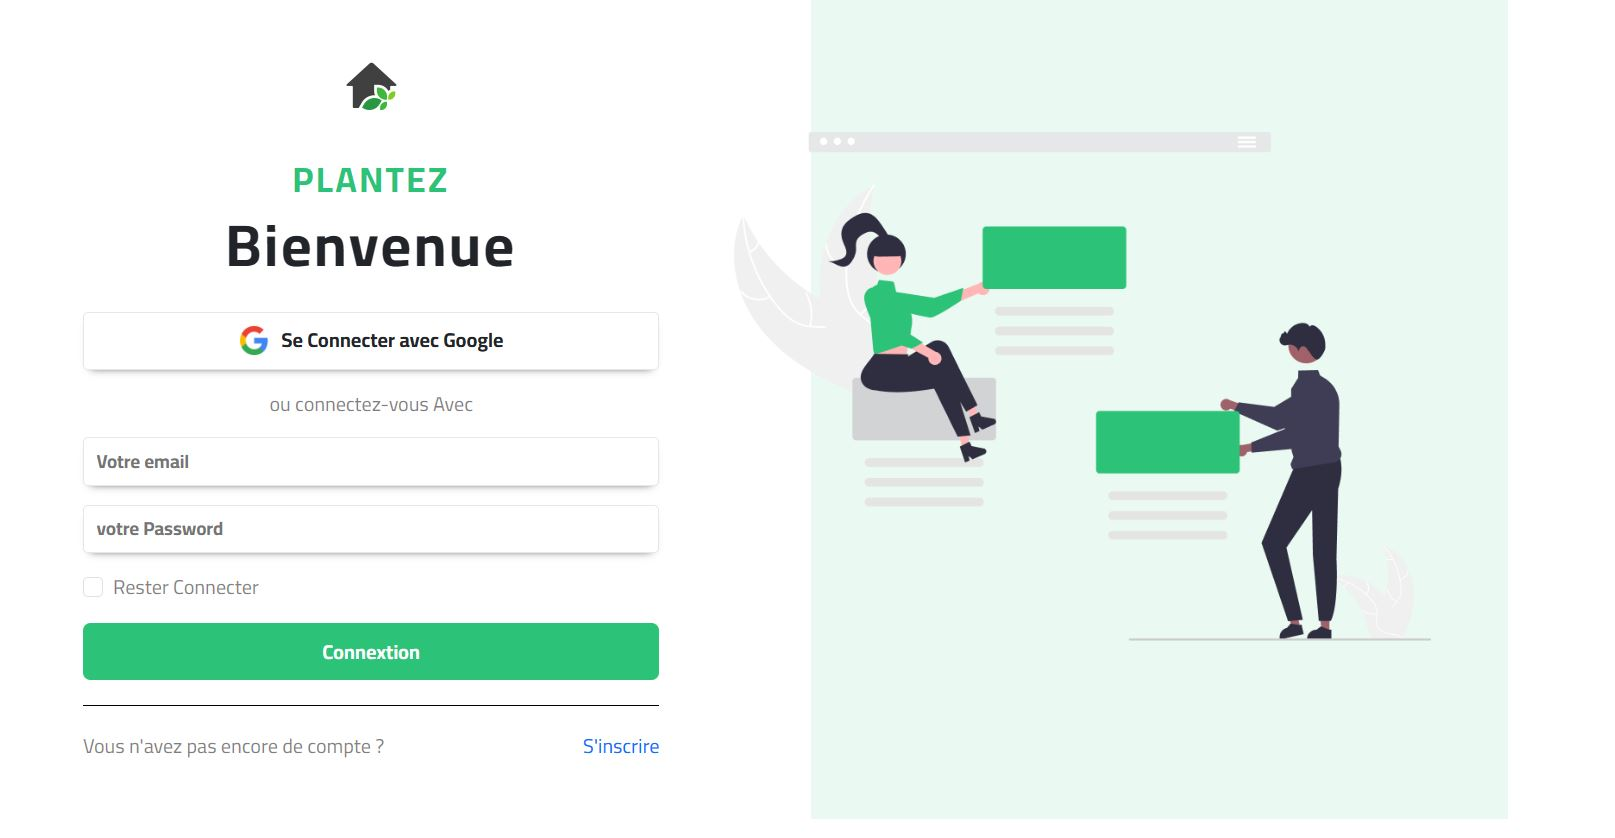
\includegraphics[width=1\textwidth]{login}
		\end{figure}
		
		\begin{figure}[h]
		\centering
  		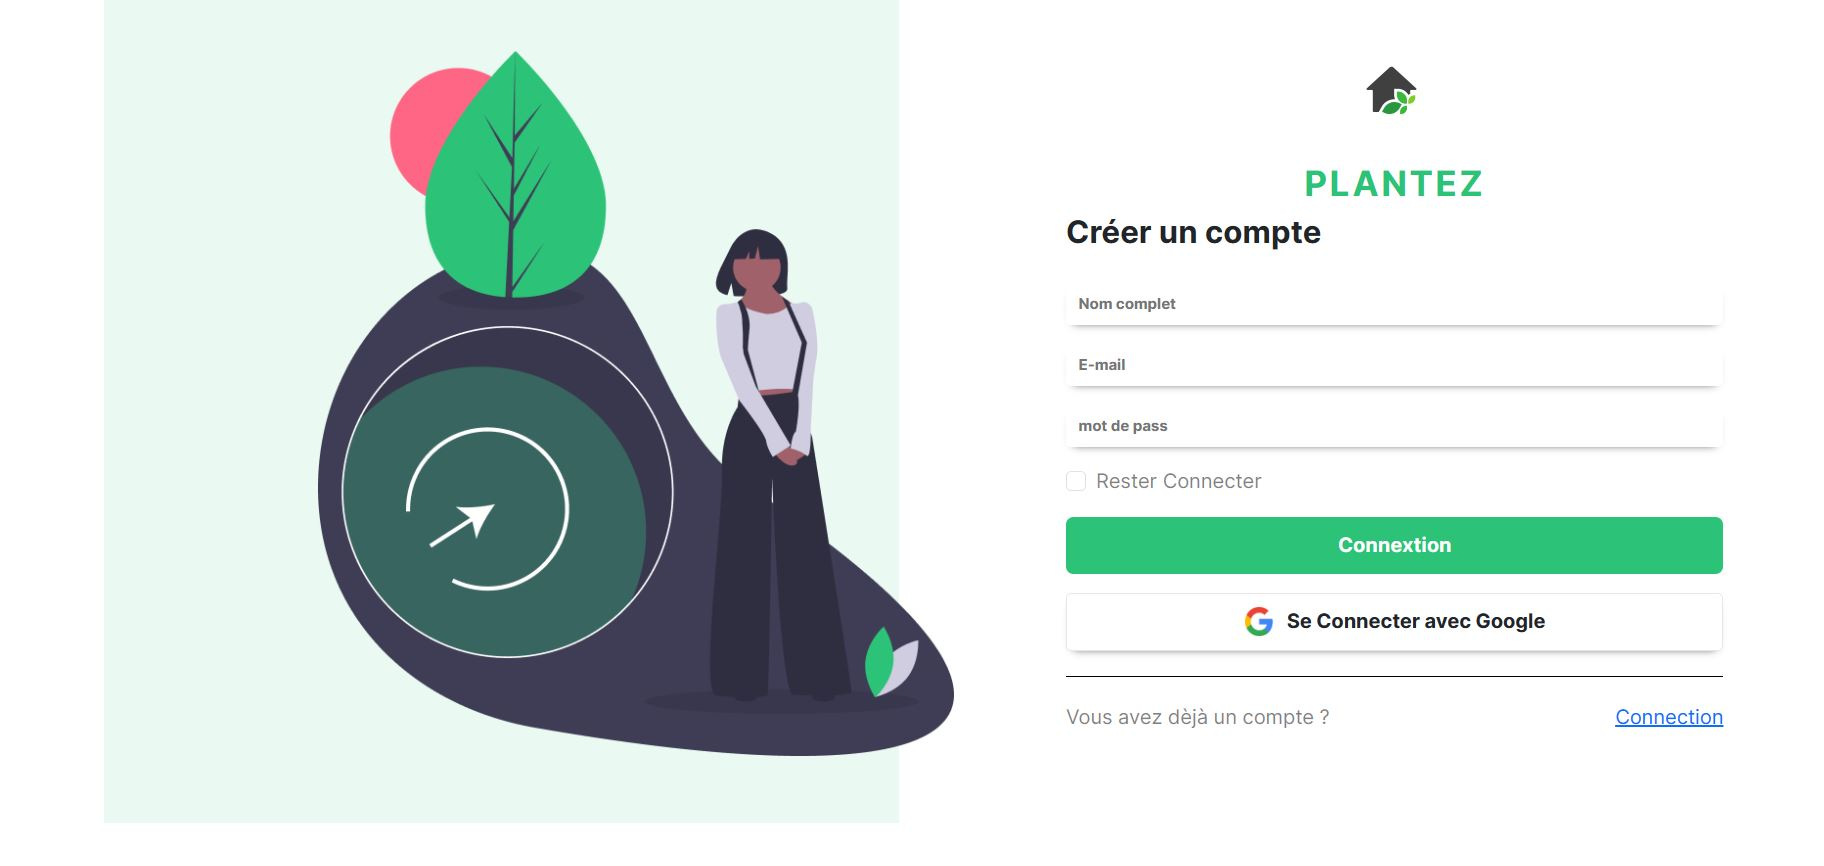
\includegraphics[width=1\textwidth]{signup}
		\end{figure}
	\newpage
		\item Après l’athentification vous pouvez consulter les pages precédentes .
		
		
		\begin{figure}[h]
		\centering
  		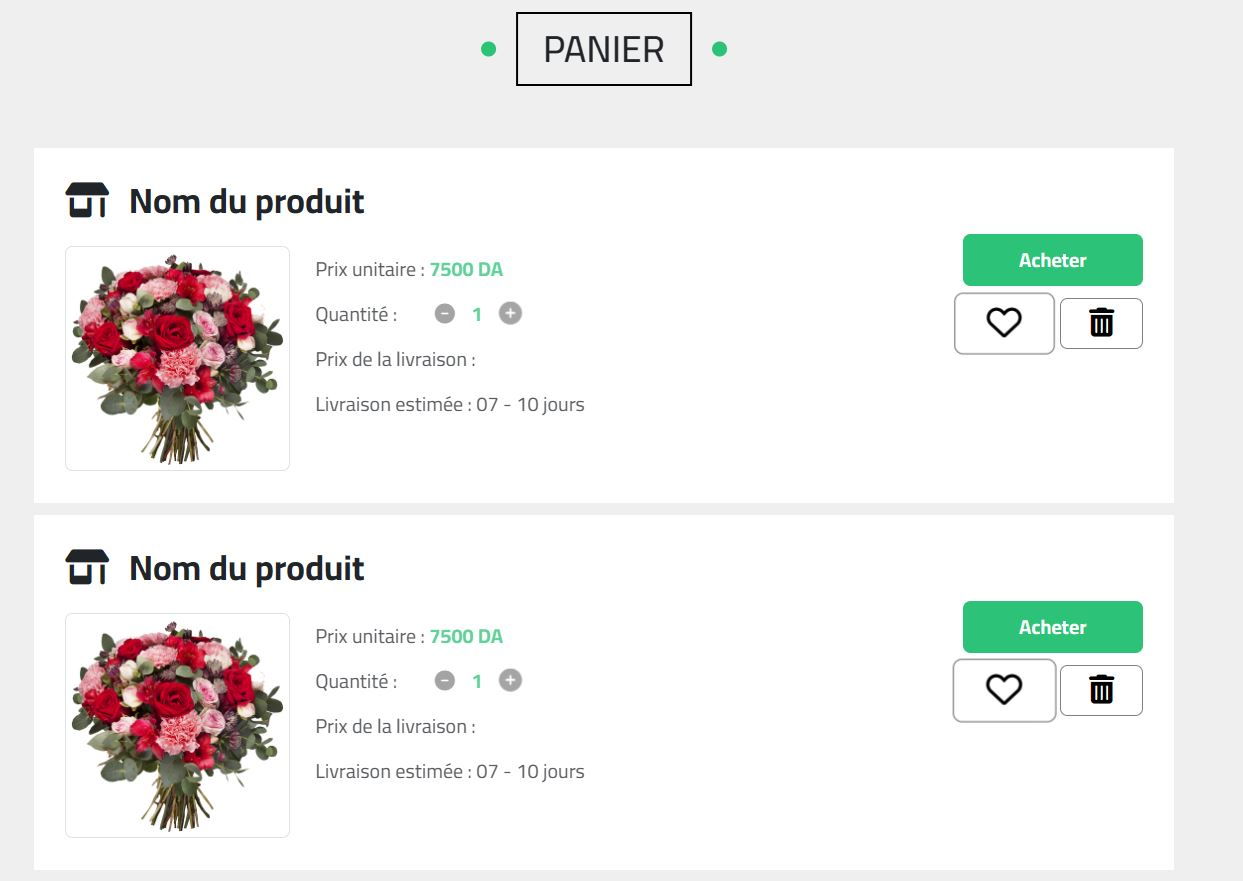
\includegraphics[width=12cm]{panier}
  		\end{figure}
  		
  		
  		\begin{figure}[h]
  		\centering
  		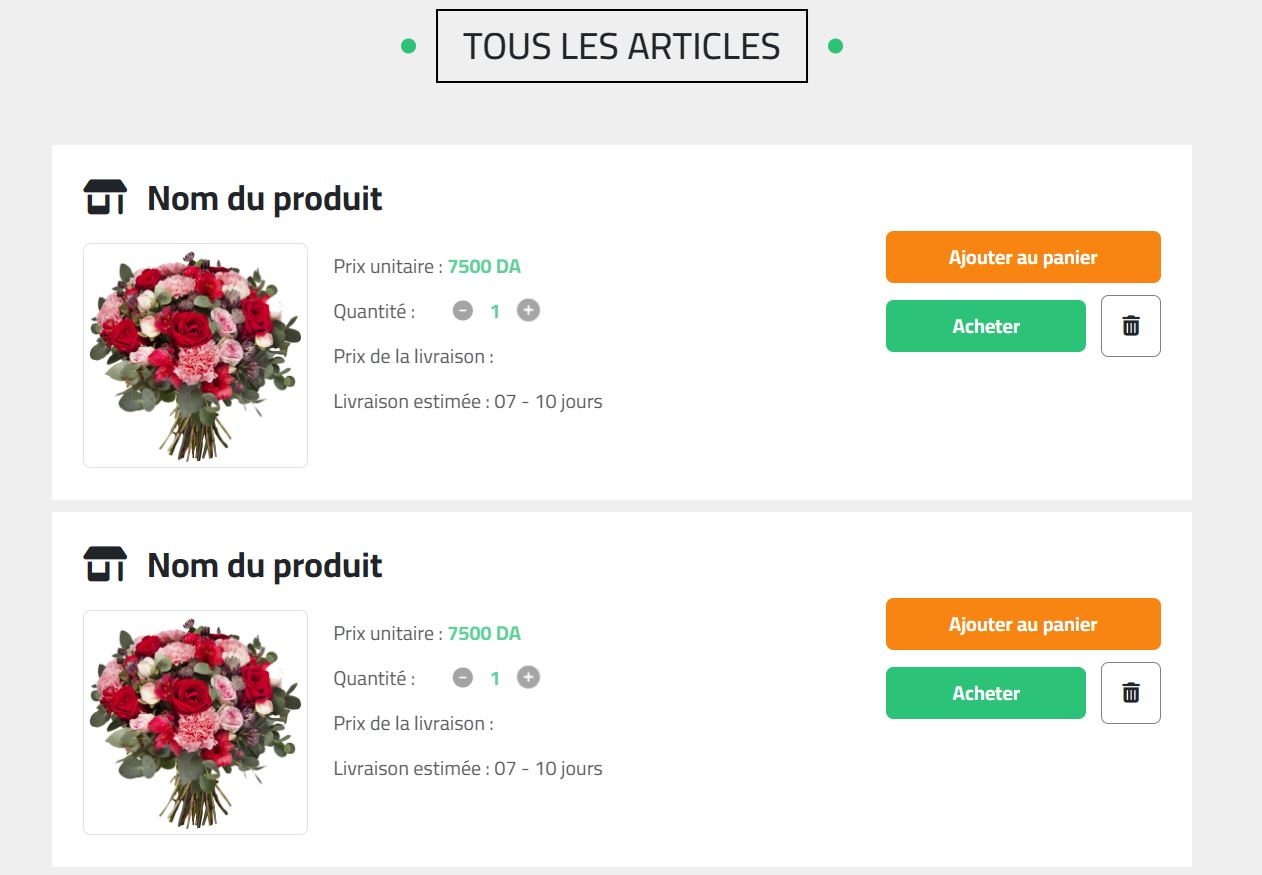
\includegraphics[width=12cm]{fav}
		\end{figure}
		
		\newpage
		
		\item A propos de nous : Dans ce champ vous allez trouver une description complète et globale sur la pipiniere avec des
différents services .
		\begin{figure}[h]
  		\centering
  		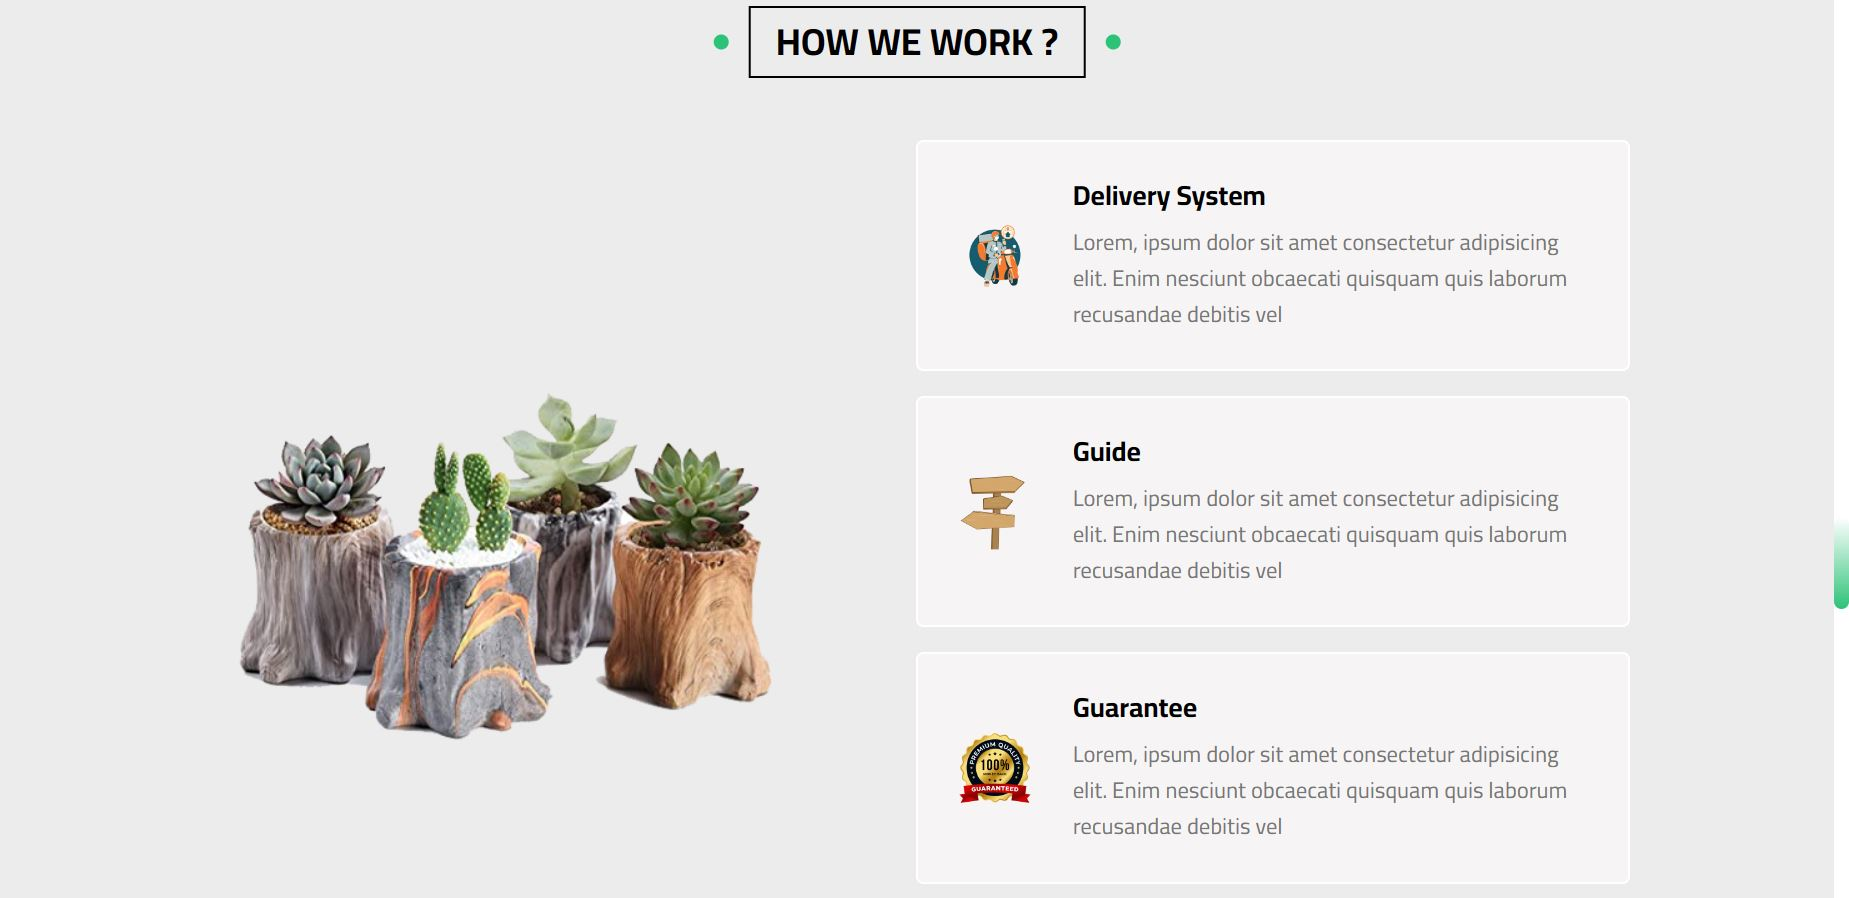
\includegraphics[width=1\textwidth]{howWeWork}
		\end{figure}
		
		\item Notre Galerie : Ici vous trouvez quelques photos de nos plantes .
		\begin{figure}[h]
  		\centering
  		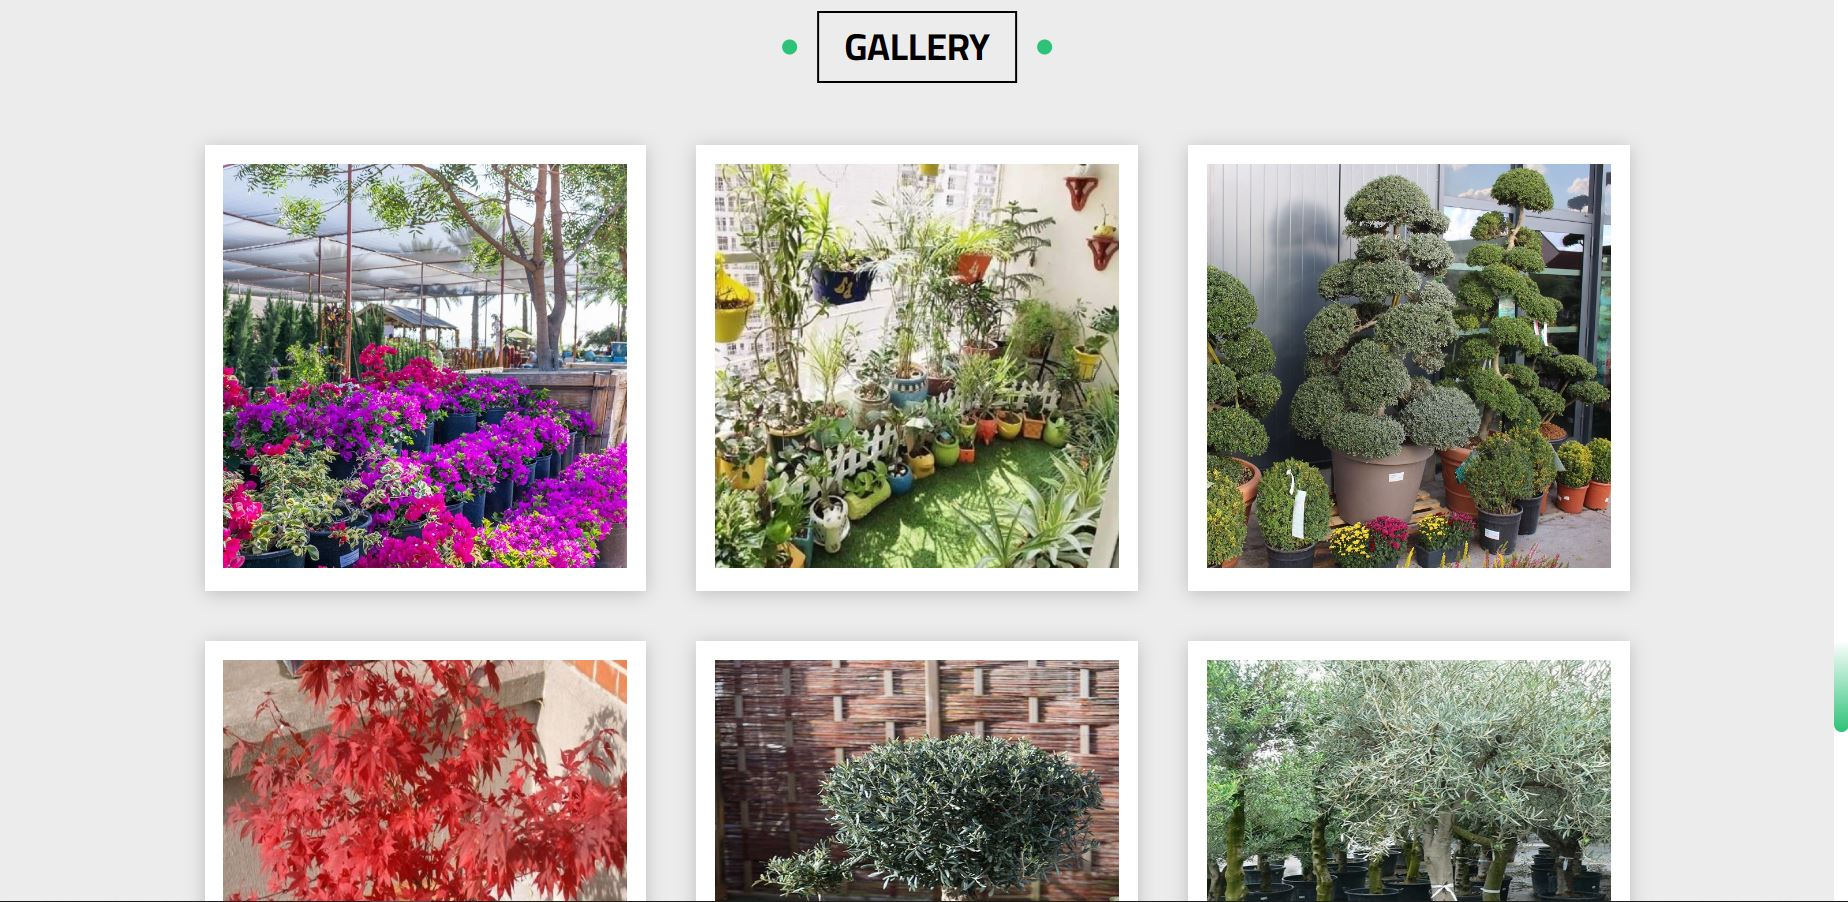
\includegraphics[width=1\textwidth]{gallery}
		\end{figure}
		
		\newpage
		\item Enfin, une zone de contact pour assurer une communication fluide entre les deux
Cotés.
		\begin{figure}[h]
  		\centering
  		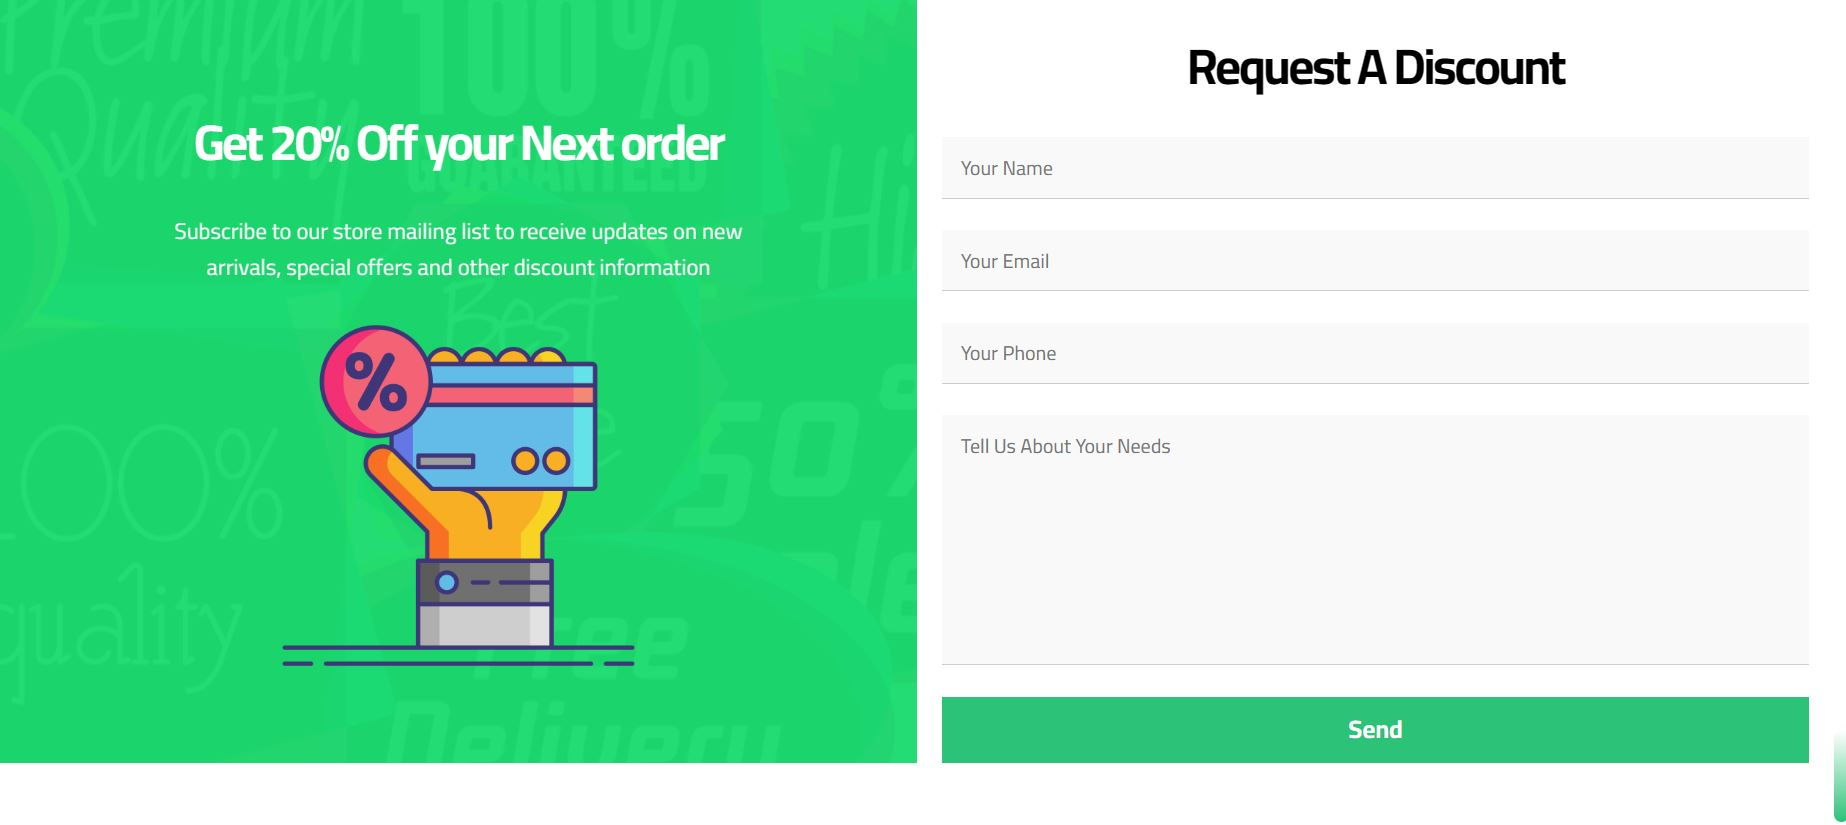
\includegraphics[width=1\textwidth]{contact}
		\end{figure}
		
		\item Footer : Dans le footer on a des raccourcis des pages précédentes : Accueil, nos
services,les categories ,les produit , à propos de nous, notre galerie contactez-nous.
Vous allez trouver aussi les différentes informations de nos contacts (les numéros, l’email) et la localisation et nos réseaux sociaux (Facebook,
Instagram).
		\begin{figure}[h]
  		\centering
  		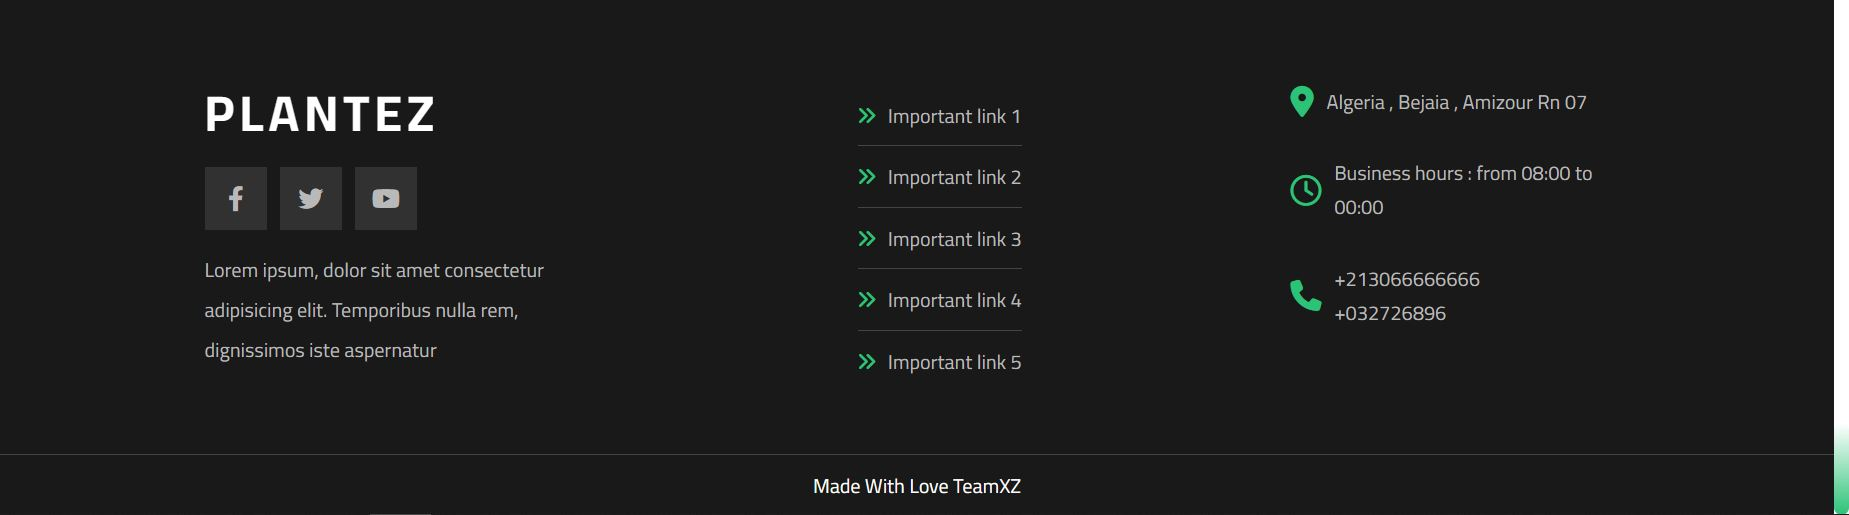
\includegraphics[width=1\textwidth]{footer}
		\end{figure}
		
		
  	\end{itemize}
  \newpage
  	\item Interfaces admin :
  	
  	\begin{itemize}
  	\item Pour le coté administrateur nous avons fait une interface simple a utilisé .Au début l’administrateur
doit se connecter avec son email et leur mot de passe apres avoir entre le lien
		\begin{figure}[h]
  		\centering
  		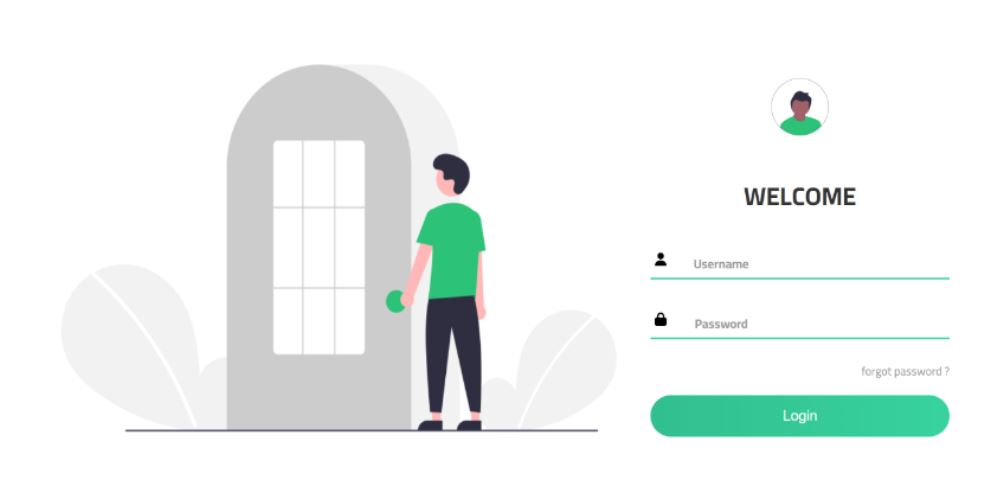
\includegraphics[width=1\textwidth]{adminlogin}
		\end{figure}
		
		\item Ensuite, l’administrateur a également la possibilité de voir le tableau de board qui contient en
générale les statistique de magasin(offres disponibles et le nombre total de commandes, produits,
catégories, et e-mail envoyès).
		\begin{figure}[h]
  		\centering
  		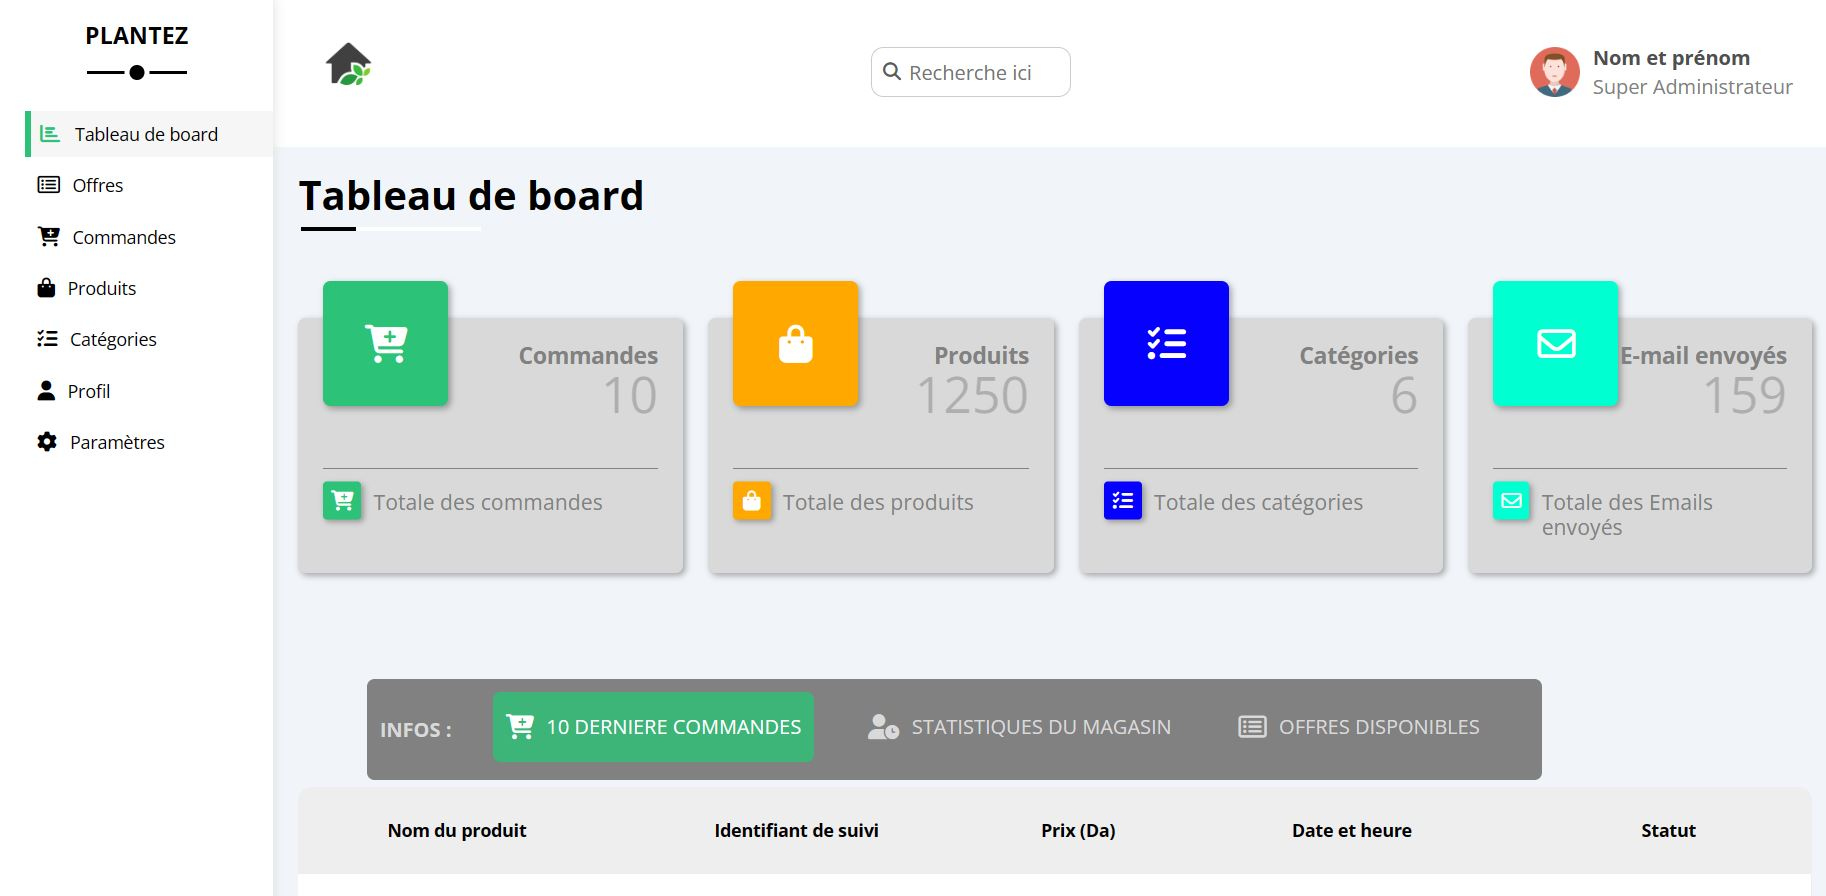
\includegraphics[width=1\textwidth]{DASH1}
  		\caption{La page d'accueil du tableau de board}
		\end{figure}
		\newpage
		\begin{figure}[h]
  		\centering
  		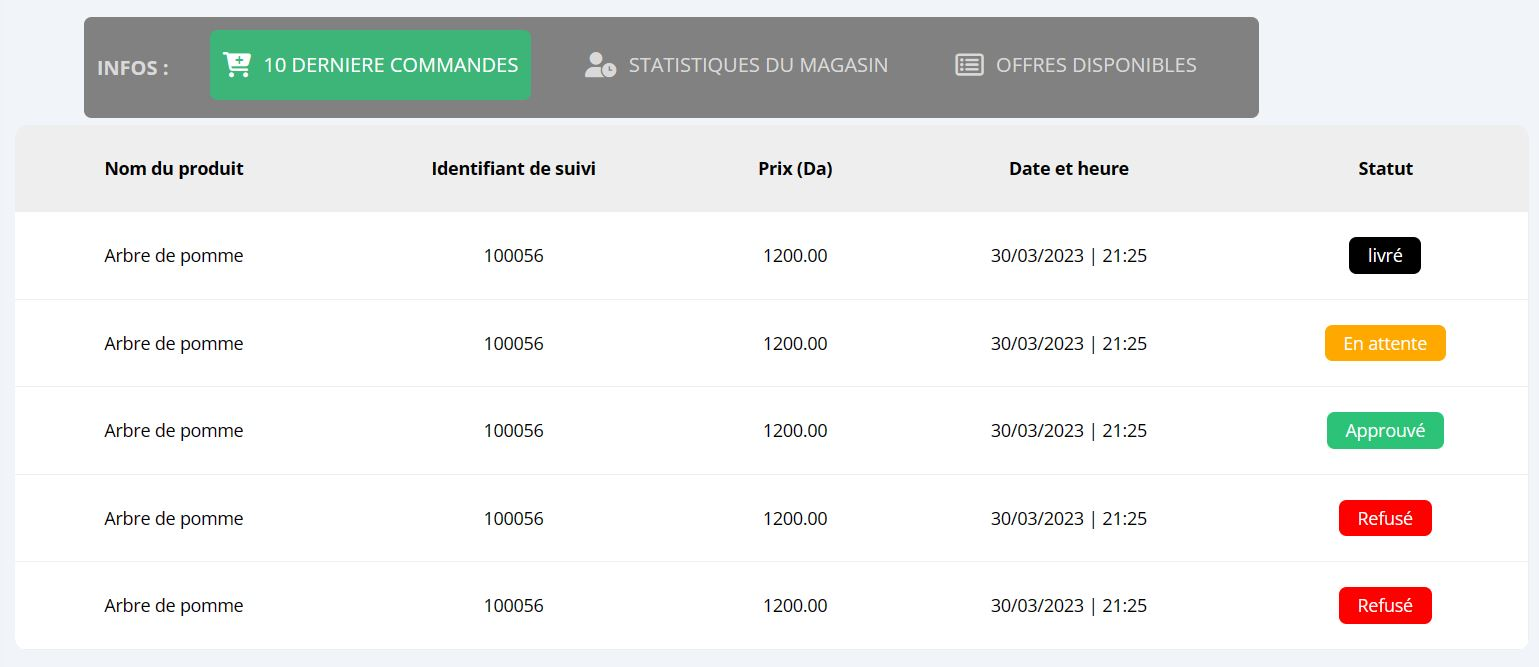
\includegraphics[width=1\textwidth]{dash2}
  		\caption{Les 10 dernières commandes  }
		\end{figure}
		\begin{figure}[h]
  		\centering
  		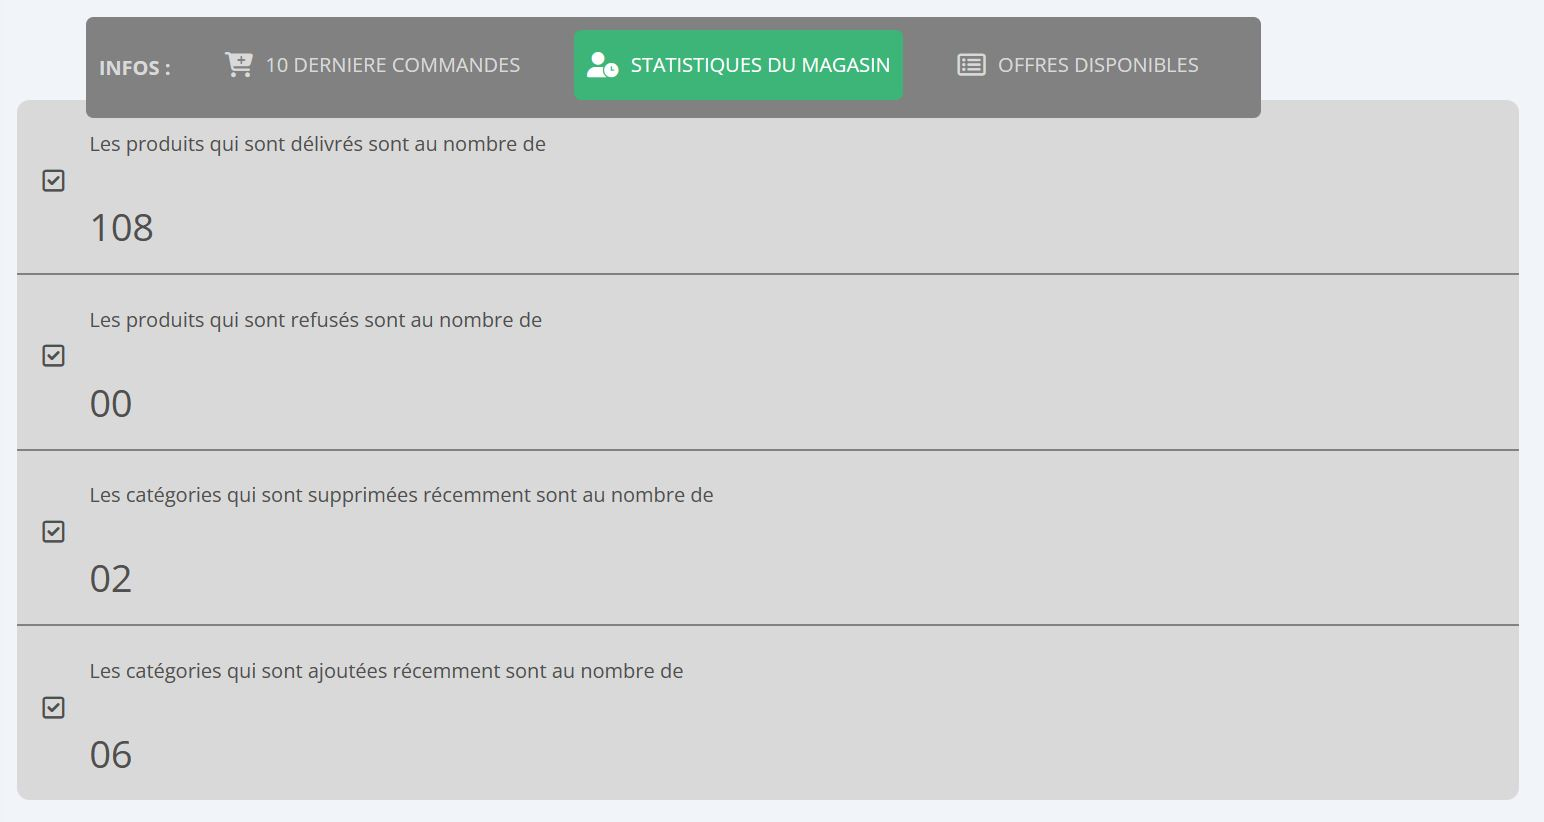
\includegraphics[width=1\textwidth]{dash3}
  		\caption{Les statistiques du magasin}
		\end{figure}
		\newpage
		\begin{figure}[h]
  		\centering
  		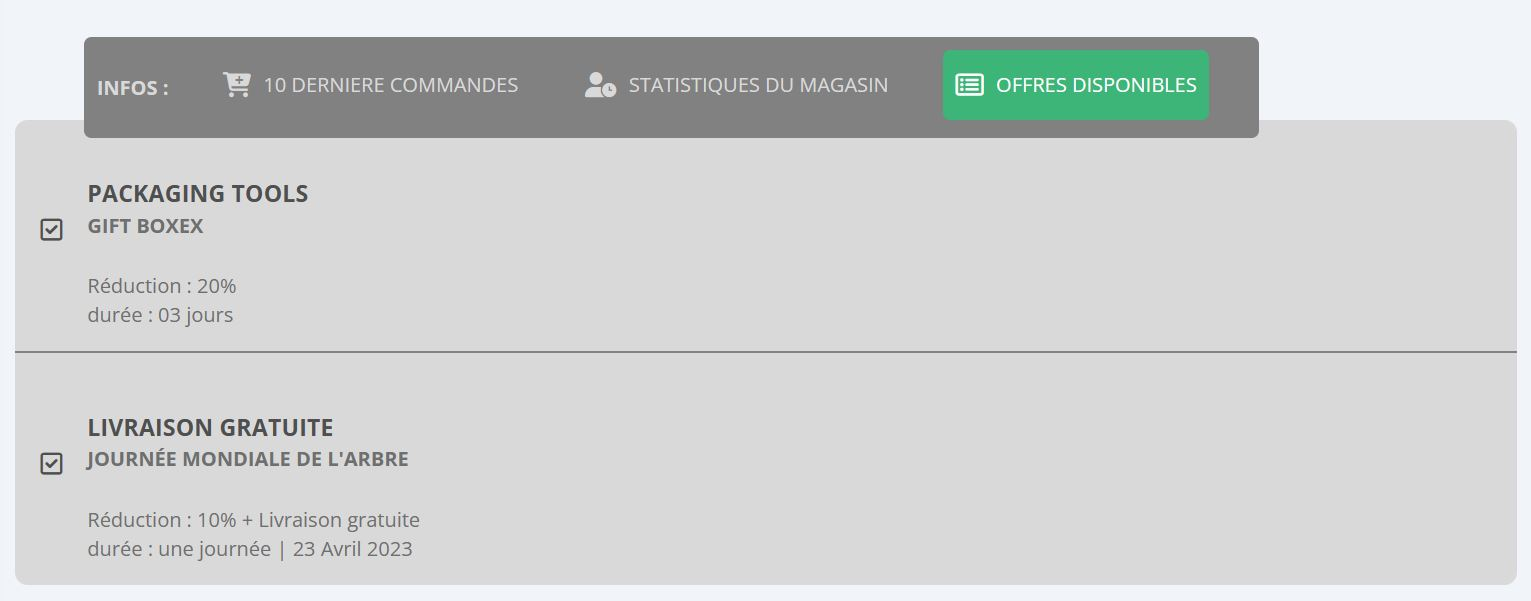
\includegraphics[width=1\textwidth]{dash4}
  		\caption{Les offres disponibles}
		\end{figure}
		
		\item Commandes: C’est la page qui contient la liste des commandes envoyees par les clients dans laquelles il peut les
accepter ou les refuser.
		\begin{figure}[h]
  		\centering
  		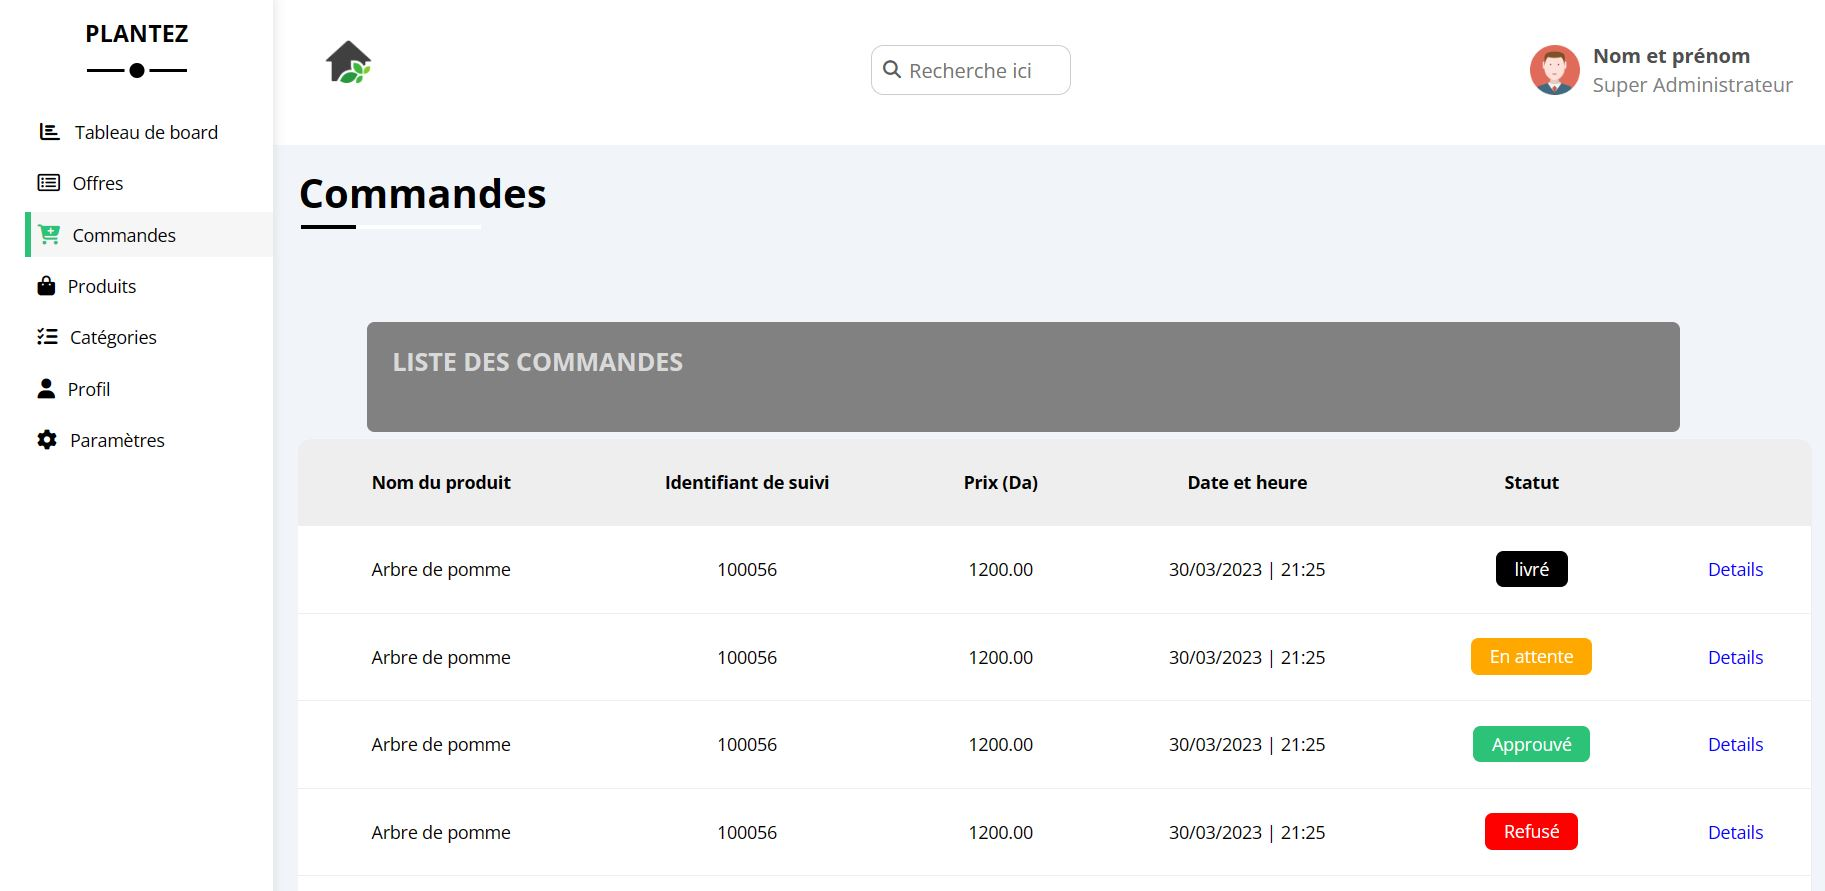
\includegraphics[width=1\textwidth]{commandes}
		\end{figure}
		
	\newpage
	
		\item Offres , catégories , produits :
Ces pages contiennent la liste des offres disponibles (resp catégories et produits )
		\begin{figure}[h]
  		\centering
  		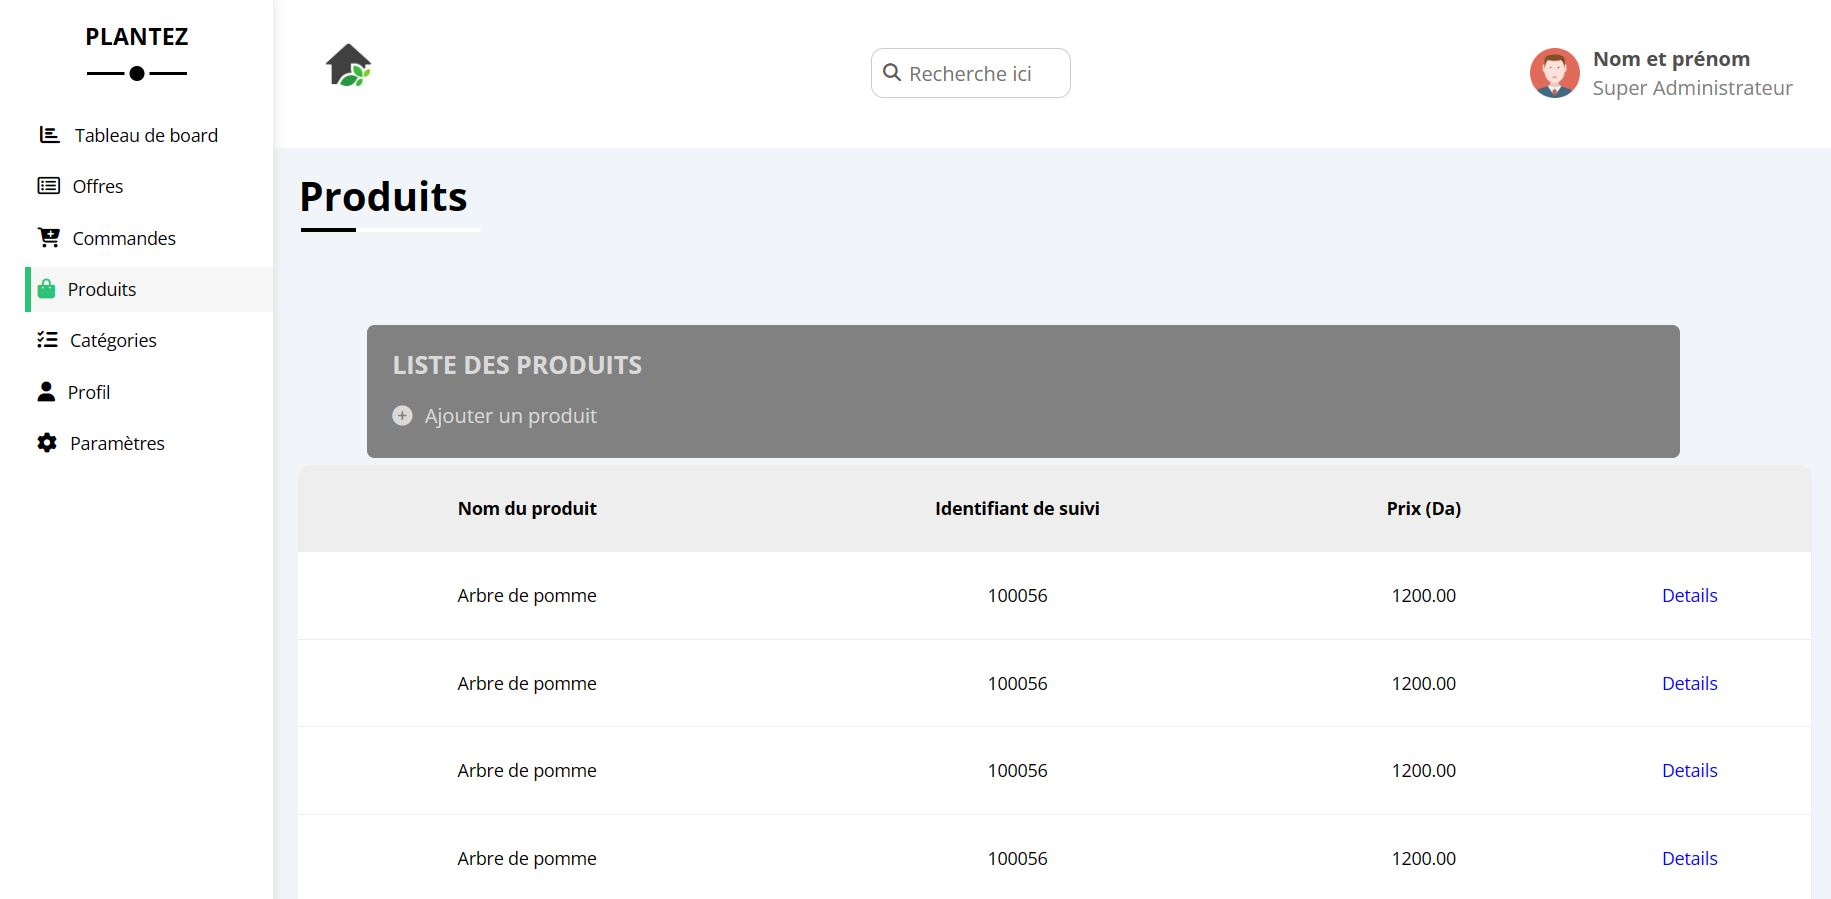
\includegraphics[width=1\textwidth]{produits}
  		\caption{Liste des produits}
		\end{figure}
	
		\begin{figure}[h]
  		\centering
  		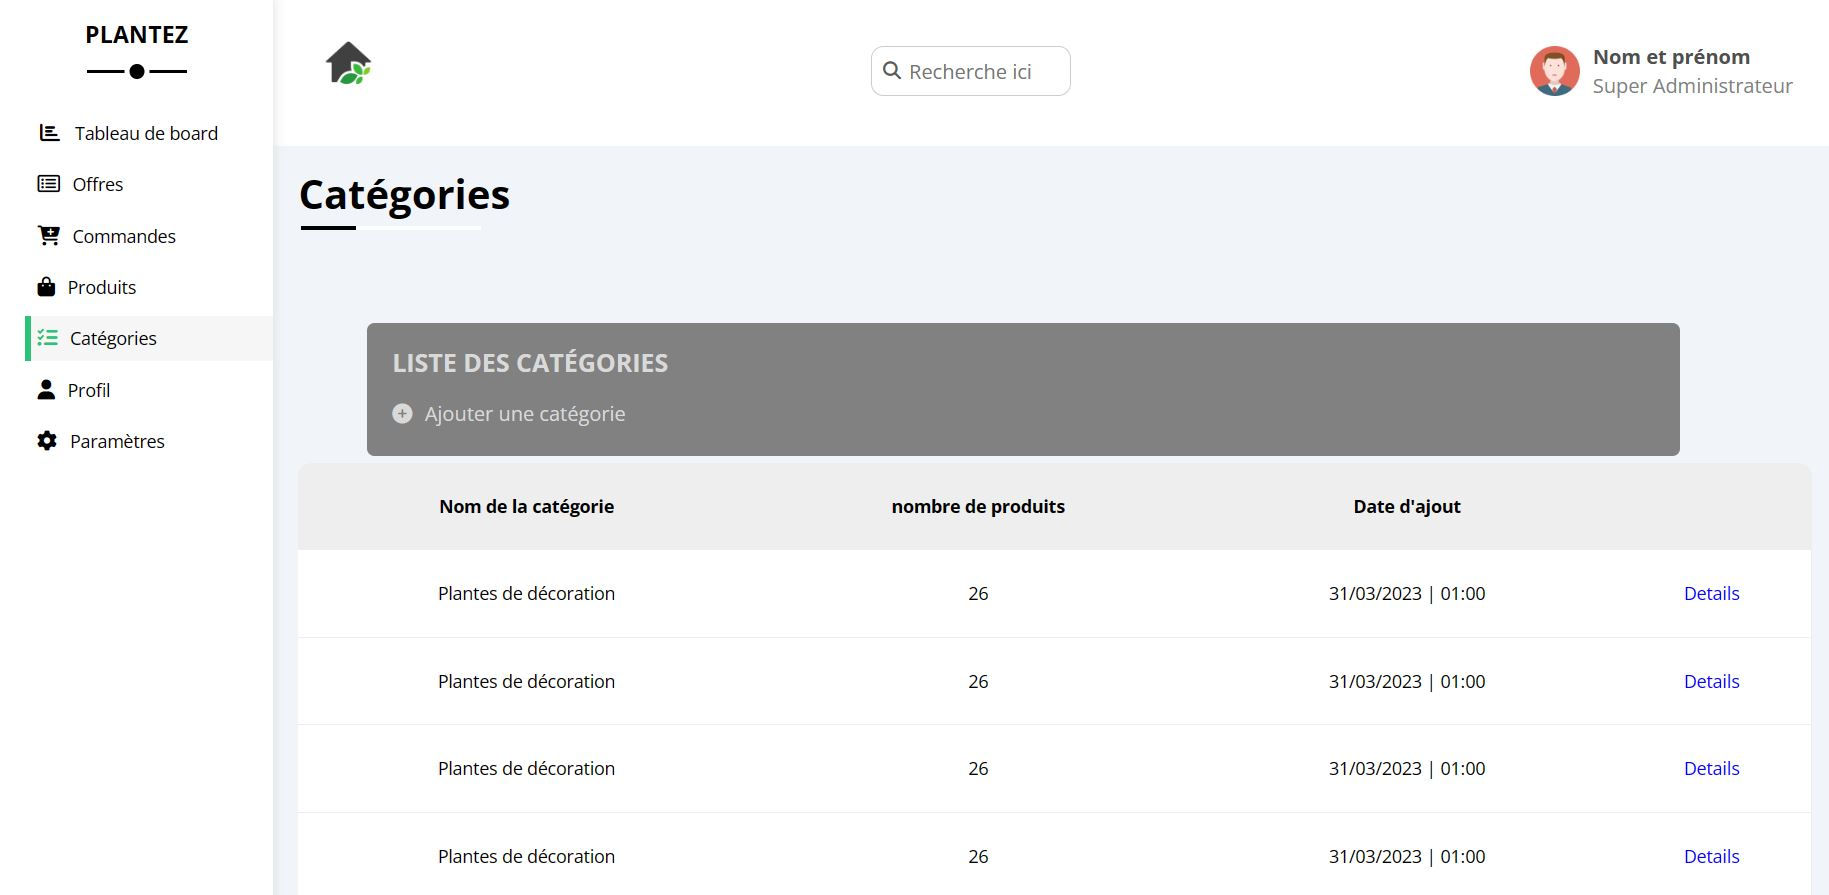
\includegraphics[width=1\textwidth]{cat}
  		\caption{Liste des catégories}
		\end{figure}
		
		\newpage
		\item L’admin peut ajouter, supprimer et modifier les informations précédentes en remplir les formulaires
suivantes :
		\begin{figure}[h]
  		\centering
  		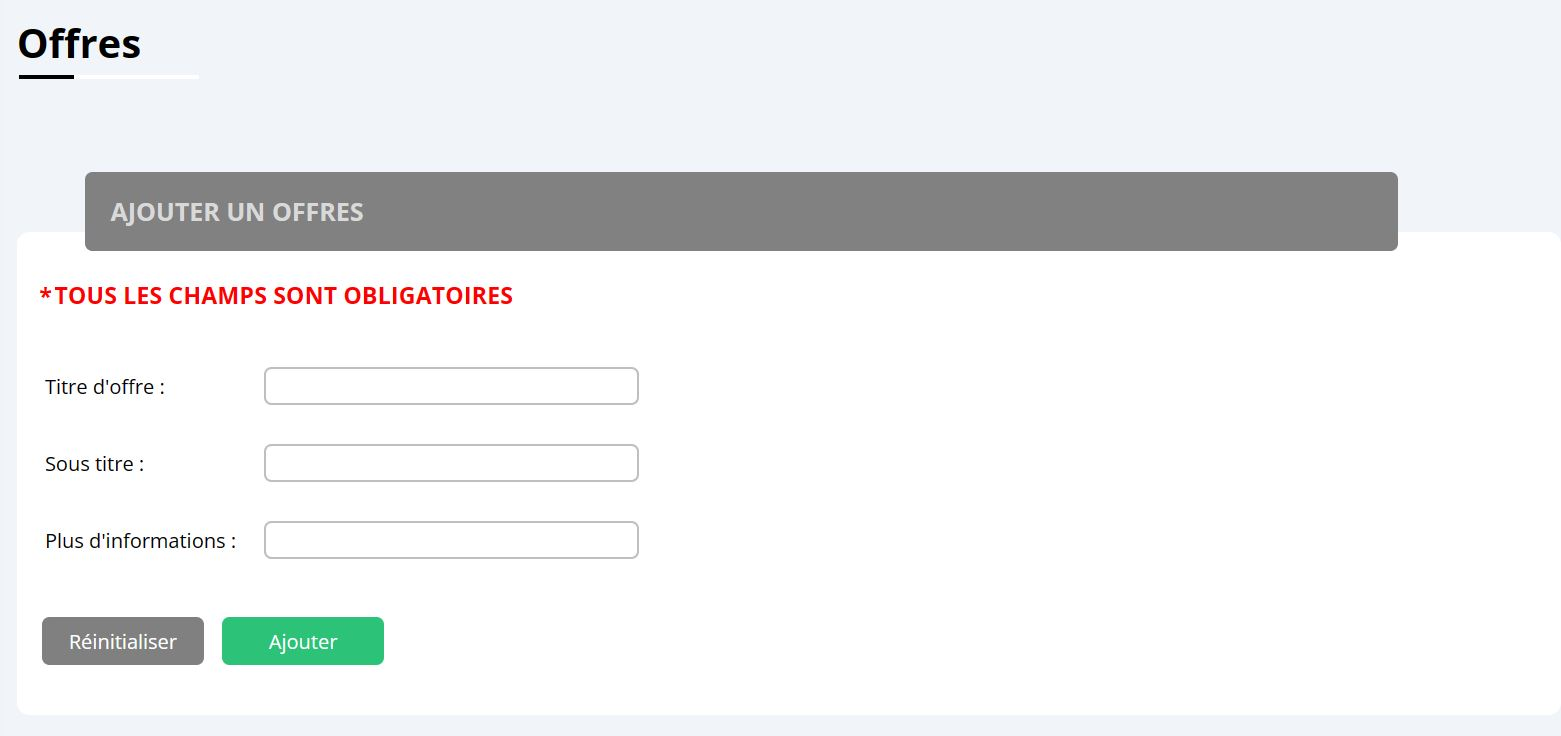
\includegraphics[width=1\textwidth]{ajtoffre}
  		\caption{Formulaire: Ajouter un offre}
		\end{figure}
		
		\begin{figure}[h]
  		\centering
  		\includegraphics[width=1\textwidth]{Ajtprod}
  		\caption{Formulaire: Ajouter un produit}
		\end{figure}
		\newpage
		
		\begin{figure}[h]
  		\centering
  		\includegraphics[width=1\textwidth]{Ajtcat}
  		\caption{Formulaire: Ajouter une catégorie}
		\end{figure}
		
		\item Profile : Cette page contient les informations personnels de l’admin (e-mail, nom complet, numero de
téléphone….), les informations de de facturations , ses réseaux sociaux et la localisation de sa
pépinière .
		\begin{figure}[h]
  		\centering
  		\includegraphics[width=12cm]{profil}
  		\caption{Profil}
		\end{figure}
		
		\item Parametre :
Enfin ,il peux accederer au parametre pour voir ces informations , modifier son mot de passe et le
numéro de téléphone après remplir ces formulaires , et pour se déconnecter .
\newpage

		\begin{figure}[h]
  		\centering
  		\includegraphics[width=1\textwidth]{param1}
  		\caption{Paramètres}
		\end{figure}
		
		\begin{figure}[h]
  		\centering
  		\includegraphics[width=1\textwidth]{param2}
  		\caption{Paramètres}
		\end{figure}

\item Conclusion :
Pour conclure ce manuel d’utilisation, nous espérons d’abord que notre projet
a pu répondre aux objectifs cités dans le cahier de charge fourni a savoir la
création d’un outil informatique (site web) pour la vente des plantes en ligne
et nous souhaitons aussi que vous avez bien compris les détails et les étapes
d’utilisation de notre site.




  	\end{itemize}
\end{enumerate}







\newpage
\section{Conclusion générale}
{\fontsize{15}{20}\selectfont 
\hspace{1cm} Dans l'ensemble, ce rapport a présenté une étude approfondie sur la conception d'un système de gestion de magasin en ligne. Nous avons commencé par l'analyse des besoins du système, suivi de la modélisation des différents aspects du système à l'aide de diagrammes de séquence et de diagrammes de classe. Nous avons également examiné les fonctionnalités du système du point de vue des utilisateurs et des responsables, et discuté des différents types de données impliqués dans le système.

En fin de compte, il est important de souligner que la conception d'un système de gestion de magasin en ligne est une tâche complexe qui nécessite une attention particulière aux détails et une compréhension approfondie des besoins des utilisateurs. En utilisant les méthodes et les outils présentés dans ce rapport, nous avons pu créer un système qui répond à ces besoins de manière efficace et conviviale.

Nous espérons que ce rapport a été utile pour comprendre les différentes étapes de la conception d'un système de gestion de magasin en ligne, et nous sommes convaincus que ce système sera bénéfique pour les utilisateurs et les responsables impliqués dans la gestion d'un magasin en ligne.

}
\section{Bibliographie/Webographie}
{\fontsize{15}{20}\selectfont
\begin{enumerate}
  	\item Front-End :
  		\begin{itemize}
        \item[] $\bullet$ https://elzero.org
    		\item[] $\bullet$ https://stackoverflow.com
    		\item[] $\bullet$ https://colorhunt.com
    		\item[] $\bullet$ https://fontawesome.com
    		\item[] $\bullet$ https://chatgpt.com
        \item[] $\bullet$ Quelques chaines youtube     
    		\end{itemize} 
 	\item Back-end : 
 		\begin{itemize}
        \item[] $\bullet$ https://expressjs.com
    		\item[] $\bullet$ https://npmjs.com
    		\item[] $\bullet$ https://nodejs.org
    		\item[] $\bullet$ https://chatgpt.com
    		\item[] $\bullet$ https://momentjs.com
        \item[] $\bullet$ Quelques chaines youtube     
    		\end{itemize} 
  	\item La diapo de présentation : 
  	 	\begin{itemize}
        \item[] $\bullet$ https://www.canva.com
        \item[] $\bullet$ Photoshop
        \item[] $\bullet$ Figma     
    		\end{itemize} 
	\item Le rapport et le cahier de charge :	
		\begin{itemize}
        \item[] $\bullet$ Latex
        \end{itemize}
\end{enumerate}

}

\section{Résumé/traduction}
{\fontsize{15}{20}\selectfont
\hspace{1cm} Le présent rapport a présenté la conception d'un système de gestion de magasin en ligne. Le système permet aux clients de parcourir et d'acheter des produits en ligne. Il permet également aux responsables de gérer les produits, les commandes, les clients et les employés.

Le rapport a commencé par la spécification des besoins, où les exigences fonctionnelles et non fonctionnelles du système ont été définies. Ensuite, les diagrammes de séquence ont été utilisés pour modéliser les principales fonctionnalités du système, notamment l'authentification, l'ajout de produits et l'achat de produits.

Le chapitre suivant a présenté les diagrammes de classes, qui décrivent la structure du système en termes d'objets, d'attributs et de méthodes. Les classes principales incluent les produits, les commandes, les clients et les employés.

Enfin, le rapport a conclu par la mise en évidence de l'importance de la mise en œuvre du système de gestion de magasin en ligne pour les entreprises qui cherchent à se développer dans l'économie numérique. Le système permet d'offrir une expérience de magasinage plus pratique et plus accessible aux clients, tout en permettant aux responsables de mieux gérer les opérations de leur entreprise.


}




\end{document}


